\documentclass[usenames,dvipsnames,table]{beamer}

\usetheme{CambridgeUS}
\usecolortheme{dolphin}

\usepackage[spanish]{babel}
\usepackage[utf8]{inputenc}
\usepackage[T1]{fontenc}
\usepackage{pgfpages}
\usepackage{relsize}
\usepackage[style=authortitle]{biblatex}
\usepackage{epigraph}
% \usepackage[table,dvipsnames]{xcolor}
\usepackage{caption}
\usepackage[labelformat=simple,subrefformat=simple]{subcaption}
\usepackage[capitalise, noabbrev]{cleveref}
\usepackage[normalem]{ulem}
\usepackage{xfrac}
\usepackage{siunitx}
\usepackage{booktabs}
\usepackage{multirow}

\usepackage{tikz}
\usetikzlibrary{shapes}
\usetikzlibrary{arrows}

% \setbeameroption{show notes on second screen=right}

\setbeamertemplate{caption}{\raggedright\insertcaption\par}
\setbeamerfont{caption}{size=\scriptsize}
\setbeamertemplate{navigation symbols}{}

\graphicspath{{figures/}}

\addbibresource{sna.bib}
\addbibresource{presentation_sna.bib}

\renewcommand\thesubfigure{(\Alph{subfigure})}

\DeclareMathOperator{\rank}{rank}
\DeclareMathOperator{\cov}{cov}

\DeclareMathOperator{\calls}{calls}
\DeclareMathOperator{\etime}{time}
\DeclareMathOperator{\sms}{sms}
\DeclareMathOperator{\contacts}{contacts}

\DeclareMathOperator{\ein}{in}
\DeclareMathOperator{\out}{out}

\DeclareMathOperator{\low}{low}
\DeclareMathOperator{\high}{high}

\DeclareMathOperator{\train}{train}
\DeclareMathOperator{\test}{test}

\DeclareMathOperator{\Betasim}{\mathcal{B}}

\DeclareMathOperator{\Precision}{Precision}
\DeclareMathOperator{\Recall}{Recall}
\DeclareMathOperator{\InvPrecision}{Inverse\ Precision}
\DeclareMathOperator{\InvRecall}{Inverse\ Recall}
\DeclareMathOperator{\Accuracy}{Accuracy}

\DeclareMathOperator{\ego}{Nbr}
\DeclareMathOperator{\cat}{Cat}

\DeclareMathOperator{\incalls}{incalls}
\DeclareMathOperator{\outcalls}{outcalls}
\DeclareMathOperator{\insms}{insms}
\DeclareMathOperator{\outsms}{insms}
\DeclareMathOperator{\intime}{outtime}
\DeclareMathOperator{\outtime}{outtime}
\DeclareMathOperator{\incontacts}{incontacts}
\DeclareMathOperator{\outcontacts}{outcontacts}


\newcommand{\ct}[1]{\multicolumn{1}{c}{#1}}
\newcommand{\meight}{\!\!\!\!\!\!\!\!}
\newcommand{\NA}{---}

\title[Ciencia de Redes]{Ciencia de Redes (Humanas y Sociales)}
\subtitle{Clase \#5}

\author{Carlos Sarraute}

\date{Abril - Junio 2019}

\institute[Grandata]{Grandata}

\begin{document}

\begin{frame}
	\hypersetup{pageanchor=false}
	\titlepage{} 
	\hypersetup{pageanchor=true}
\end{frame}

\section{Introducción}


\begin{frame}{Introducción}

	Las operadores de telecomunicaciones tienen acceso a una gran cantidad de información sobre las comunicaciones y habitos de sus usuarios~\footcite{huurdeman2003}, pero a pesar de eso la minería de datos de telcos a gran escala es una disciplina relativamente nueva~\footcite{han2002emerging}.

	Esta tesis usa métodos similares a los usados por Óskarsdottir et~al.~\footcite{oskarsdottir2016} y Singh et~al.~\footcite{singh2013predicting}, además de una fuente de información de una telco y de un banco grande para encontrar que la distribución de ingresos de los usuarios sigue de manera cercana (pero no exacta) la distribución de ingresos de la población en general.
\end{frame}

\section{Marco Teórico}

\subsection{Homofilia Social}

\begin{frame}{Homofilia Social}
	\epigraph{``La gente ama a los que son como sí mismos.''}{\textit{Aristoteles \\ Retórica}}
	\note{%
		La similaridad lleva a la conexión.

		La gente tiene características, como edad, género, o estatus socioeconómico, con el que hay una mayor tasa de contacto que gente disimilar.

		El trabajo hecho en esta tesis está relacionado a descubrir y explotar casos de homofilia en la población de un grafo social.
	}
\end{frame}

\begin{frame}{Homofilia Social}
	\begin{figure}
		\begin{subfigure}[b]{0.48\framewidth}
			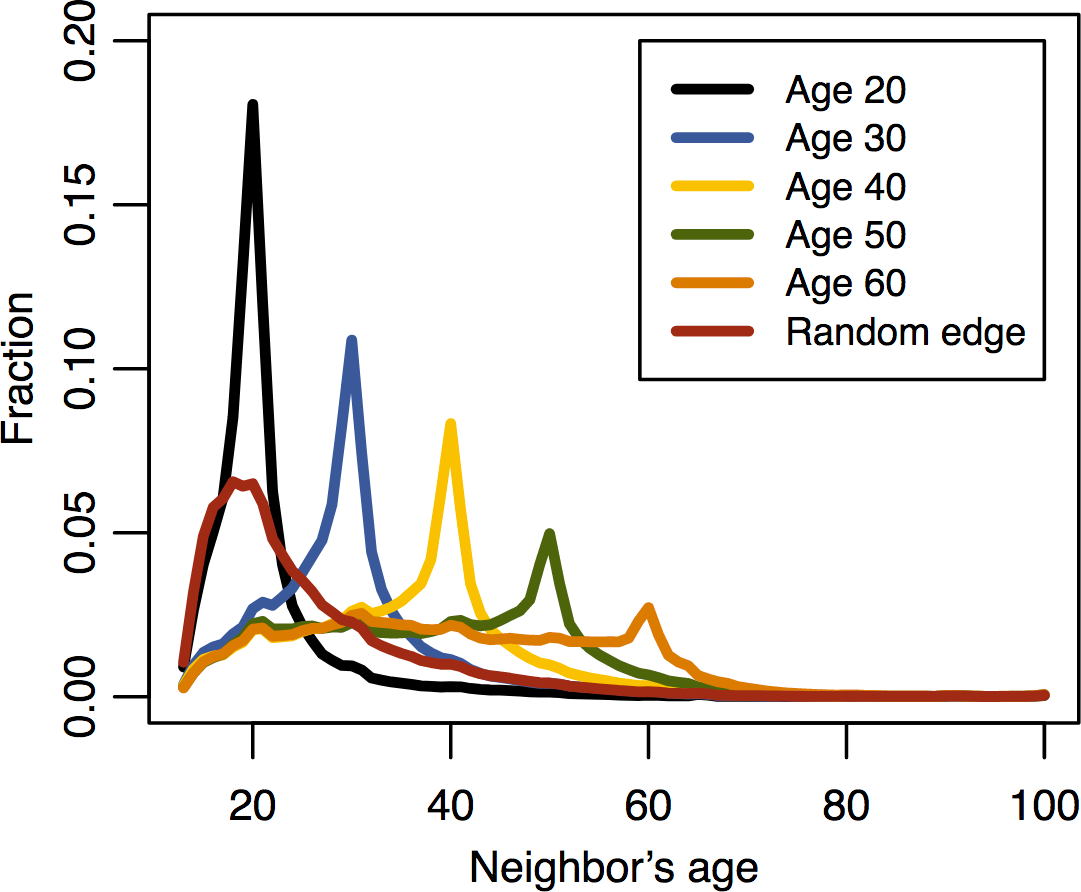
\includegraphics[width=0.9\textwidth]{age_homophily.png}
			\caption{}%
			\label{fig:age_homophily}
		\end{subfigure}
		\begin{subfigure}[b]{0.48\framewidth}
			\hfill{}
			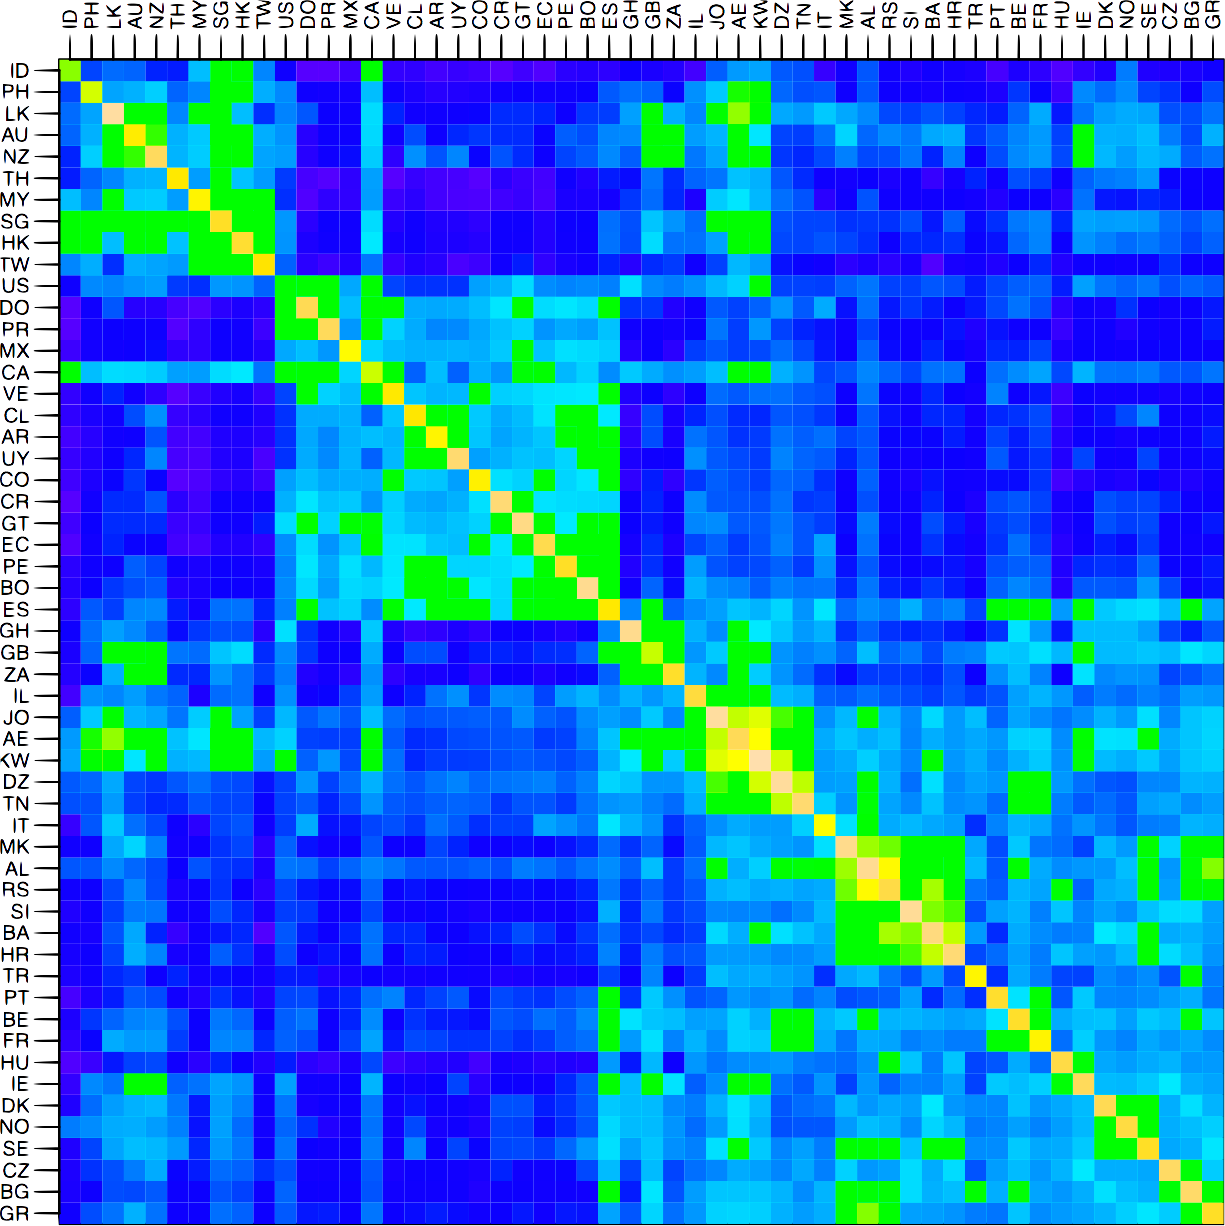
\includegraphics[width=0.9\textwidth]{country_homophily.png}
			\caption{}%
			\label{fig:country_homophily}
		\end{subfigure}
		\caption{Ejemplos varios de homofilia en un cierto grafo social\footcite{ugander2011anatomy}. \subref{fig:age_homophily}: Distribución de edades para contactos de usuarios de cada edad. \subref{fig:country_homophily}: Mapa de calor marcando la cantidad normalizada de contactos entre cada par de países.}
	\end{figure}

	\note{%
		Dos casos muy comunes de homofilia en grados sociales son la homofilia por edad y la homofilia por país. Ambas fueron investigadas por Ugander~et~al en el paper citado en este slide.

		Como se pueden apreciar en estos gráficos, el rango de edades para las conexiones de amistad en una red social están altamente sesgadas hacia la misma edad que tiene cada persona. También se puede ver lo mismo cuando se grafica los pares entre países entre todas las conexiones de amistad.
	}
\end{frame}

\subsection{Inferencia Bayesiana}

\begin{frame}{Inferencia Bayesiana}
	\parbox{.5\textwidth}{\raggedleft{}
		\begin{equation*}
			P \left( H \mid E \right) = \frac{P \left( E \mid H \right) \cdot P \left( H \right)}{P \left( E \right)}
		\label{eq:bayes}
		\end{equation*}
	}
	\hfill
	\parbox{.45\textwidth}{\raggedright{}
	\epigraph{``Dada la cantidad de veces en el que un evento desconocido sucedió y falló en suceder, la probabilidad de este pasando en una sola prueba está entre dos grados de probabilidad que pueden ser nombrados''}{\textit{Thomas Bayes \\ An Essay towards solving a Problem in the Doctrine of Changes}}
	}

	\note{%
		Parte de este trabajo usa enfoque bayesiano a las estadísticas. A diferencia del común enfoque frecuentista, donde los parámetros están fijos y desconocidos y las hipótesis son ciertas o falsas, cualquier cosa desconocida se describe con una distribución de probabilidad que describe su incertidumbre.
	}
\end{frame}

\subsection{Teorema de Bayes}

\begin{frame}{Teorema de Bayes}
	\begin{align*}
		&P \left( H \mid E \right) = \frac{P \left( E \mid H \right) \cdot P \left( H \right)}{P \left( E \right)} &\text{\textbf{Teorema de Bayes}} \\
		\vspace{4em} \\
		\onslide<1> {%
		&P \left( H \mid E \right) &\text{\textbf{Posterior Probability}} \\
		&P \left( E \mid H \right) &\text{\textbf{Likelihood}} \\
		&P \left( H \right) &\text{\textbf{Prior Probability}} \\
		&P \left( E \right) &\text{\textbf{Marginal Likelihood}}
		}
		\onslide<2> {%
			&P \left( H \mid E \right) \propto P \left( E \mid H \right) \cdot P \left( H \right) &\text{\textbf{Posterior Proportionality}}
		}
	\end{align*}
	
	\note{%
		\onslide<1>{%
			El teorema de Bayes describe la probabilidad de un evento en base a conocimiento a priori de las condiciones posiblemente relacionadas a este. Este tiene cuatro términos.
			\begin{itemize}
				\item \textbf{Posterior Probability}, que es la probabilidad condicional asignada después de que el evento se toma en cuenta. \\
				\item \textbf{Likelihood}, el grado de probabilidad de $E$ dado que $H$ es cierto. \\
				\item \textbf{Prior Probability}, las suposiciones hechas en el problema antes de los experimentos. \\
				\item \textbf{Marginal Likelihood}, la función de probabilidad donde algunos parámetros fueron marginalizados. Se usa como constante normalizante para que la \emph{Posterior Probability} integre a $1$, haciendo que sea una probabilidad válida.
			\end{itemize}
		}
		\onslide<2>{%
			Estas ecuaciones son probabilidadeso continuas, que por definición deben integrar a $1$. Por esa razón, se suele usar la ecuación en este \textit{slide}, que define la proporcionalidad del \textit{posterior}.
		}
	}
\end{frame}

\subsection{Distribución Beta}

\begin{frame}{Distribución Beta}
	\begin{align*}
		X &\sim B \left( \alpha, \beta \right) \\
		\mathrm{B} \left( \alpha, \beta \right) &= \frac{\left( \alpha + \beta - 1 \right)!}{\left( \alpha - 1 \right)! \cdot \left( \beta - 1 \right)!}
	\vspace{1em} \\
		f \left( X; \alpha, \beta \right) &= \frac{1}{\mathrm{B} \left(\alpha, \beta \right)} \cdot x^{\alpha - 1} {\left( 1 - x \right)}^{\beta - 1} \\
		\vspace{1em} \\
		F \left( X; \alpha, \beta \right) &= P \left( X \leq x \right) \\
		F \left( X; \alpha, \beta \right) &= \frac{1}{\mathrm{B} \left(\alpha, \beta \right)} \cdot \int^x_0 {t^{\alpha - 1} {\left( 1 - t \right)}^{\beta - 1} dt} \\
		\vspace{1em} \\
		Q \left( p \right) &= \inf \left\{ x \in \mathbb{R} \mid p \leq F \left( x \right) \right\}
	\end{align*}

	\note{%
		La distribución Beta es una familia de distribuciones de probabilidad paramterizada por dos parámetros $\alpha$ y $\beta$. Se suele usar para modelar como actúan variables aleatorias limitadas a intervalos de largo finito.

		En el contexto de inferencia bayesiana, la distribución Beta es el conjugate prior de la distribución binomial. Esto nos permite describir conocimientos iniciales sobre la probabilidad de éxito de una distribución bivariada.

		Dado una distribución binomial con $\alpha$ ejemplos positivos y $\beta$ ejemplos negativos como tirar una moneda $(\alpha + \beta)$ veces, la distribución Beta modela la probabilidad de que la primer distribución sea positiva.
		
		El trabajo principal de esta tesis usa mucho la función cuántil de la distribución Beta, que es la inversa de la función cumulativa de probabilidad. No hay ninguna formula cerrada para esto, pero se puede aproximar fácilmente usando el método de Newton.
	}
\end{frame}

\begin{frame}{Distribución Beta}
	
	\begin{figure}
		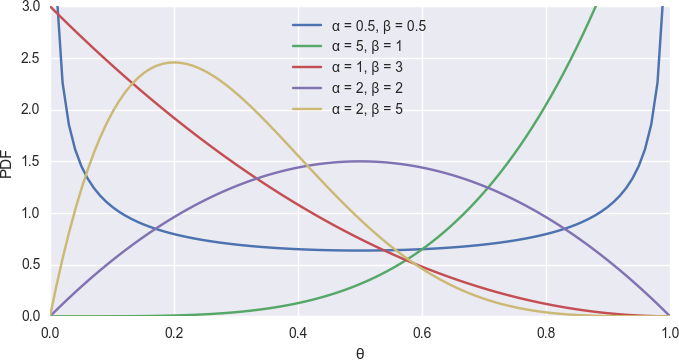
\includegraphics[width=\framewidth]{beta.png}
		\caption{Distribución Beta para diferentes valores de $\alpha$ y $\beta$.}
	\end{figure}
	
	\note{%
		Este gráfico representa la distribución Beta para diferentes valores de $\alpha$ y $\beta$.
	}
\end{frame}

\section{Fuente de Datos}

\subsection{Fuente de Datos}

\begin{frame}{Fuente de Datos}
	Esta tesis usa dos fuentes de datos principales para cierta población.
	\begin{enumerate}
		\item Dos conjuntos $P$ y $S$ con \emph{Call Detail Records} de llamadas y SMS\@.
		\item Un conjunto $B$ de datos bancarios, del cual se puede extraer el salario mensual.
	\end{enumerate}
\end{frame}

\begin{frame}{Fuente de Datos}
	Con estos datos se calcula el \emph{Grafo Social}.
	\begin{equation*}
		G = \left< \text{V}, \text{E} \right>
	\end{equation*}
	Donde $V$ contiene datos de usuarios y su nivel de ingreso (si se conoce), y $E$ contiene sus conexiones con otros usuarios. Se puede usar el grafo social para entender el comportamiento de los usuarios \footcite{gonzalez2008understanding}\footcite{ponieman2013human}\footcite{sarraute2015city}.

	\begin{center}
		\tikzstyle{att} = [circle, draw, fill=black!25, minimum size=10pt]
\tikzstyle{edge} = [draw, thick, >=latex]

\begin{tikzpicture}
	\node[att] (0) at (-2, 0) {};
	\node[att] (1) at (0, 0) {};
	\node[att] (2) at (0, -2) {};
	\node[att] (3) at (-2, -2) {};
	\node[att] (4) at (-1, -1) {};
	\node[att] (5) at (-3, -1) {};
	\path[edge, ->] (0) -- (1);
	\path[edge, ->] (1) -- (2);
	\path[edge, ->] (2) -- (3);
	\path[edge, <->] (3) -- (0);
	\path[edge, ->] (0) -- (4);
	\path[edge, <->] (4) -- (2);
	\path[edge, ->] (4) -- (3);
	\path[edge, <->] (5) -- (0);
	\path[edge, ->] (5) -- (3);

	\node[att] (a) at (1, 0) {};
	\node[att] (e) at (1, -1.5) {};
	\path[edge, <->] (1) -- (a);
	\path[edge, <-] (1) -- (e);
	\path[edge, ->] (2) edge [bend right = 30] (e);

	\path[edge, ->] (e) -- (a);
\end{tikzpicture}

	\end{center}
\end{frame}

\subsection{Inferencias Básicas}
\begin{frame}{Distribución de Ingresos por Edad}
	\begin{figure}
		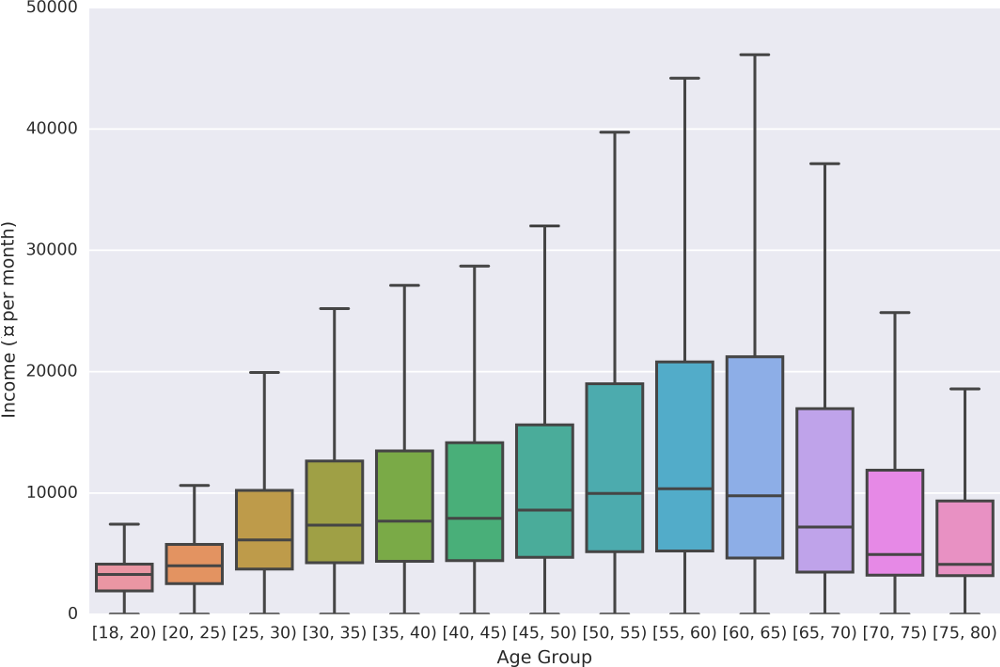
\includegraphics[width=.80\framewidth]{income_age_boxplot4.png}
		\caption{Distribución de ingresos por grupo de edad.}
	\end{figure}
\end{frame}

\begin{frame}{Distribución de Ingresos Totales}
	\parbox{.60\textwidth}{\raggedleft{}
		\begin{figure}
			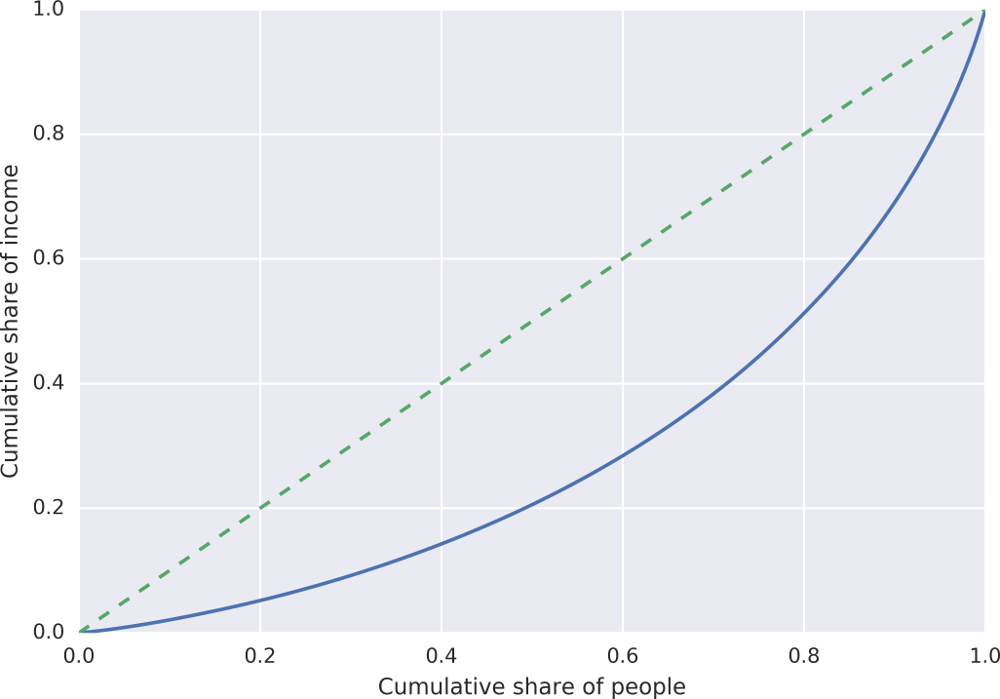
\includegraphics[width=.6\framewidth]{cumulative_income.png}
			\caption{Proporción acumulada de ingresos por proporción acumulada de la población.}
		\end{figure}
	}
	\parbox{.39\textwidth}{\raggedright{}
		Dentro de los usuarios de este banco:
		\begin{itemize}
			\item 20\% de la población tiene 50\% de los activos.
			\item Gini = 45\%.
		\end{itemize}
	}

	\note{%
		Este gráfico nota la desigual distribución de ingresos dentro de los usuarios del banco, donde la mayoría de los activos líquidos pertenecen a menos de un quinto de la población.

		El coeficiente Gini mide la desigualdad de riqueza de un grupo de gente: un valor de 0\% indica total igualdad, mientras que un valor de 100\% indica una sola persona teniendo toda la riqueza. El coeficiente en este banco es igual a 45\%, que es un poco menor al valor total de 48\% del país del estudio ya que no incluye a la población no bancarizada de este país.
	}
\end{frame}

\section{El Modelo Bayesiano}

\subsection{Introducción}

\begin{frame}{El Modelo Bayesiano}
	El objetivo principal de esta tesis es buscar un algoritmo que prediga el nivel de ingresos de un usuario dependiendo de datos sobre el \emph{Grafo Social}.

	Esto se logra aprovechando el nivel de \emph{Homofilia de Ingresos} en los usuarios.
\end{frame}


\subsection{Homofilia de Ingresos}

\begin{frame}{Coeficiente de Spearman}
	El Coeficiente de Spearman $r_s$ mide la correlación entre la distribución de dos monotónicas variables $x$ e $y$~\footcite{statistical_analysis}, donde $\rho_{x, y}$ es el \emph{Coeficiente de Pearson} entre $x$ e $y$.


	\begin{equation*}
		r_s = \rho_{\rank\left(x\right), \rank\left(y\right)} = \frac{\cov\left(\rank\left(x\right), \rank\left(y\right)\right)}{\sigma_{\rank(x)} \sigma_{\rank(y)}}
	\end{equation*}

	\onslide<2>{%
		En la fuente de datos usada para esta tesis,

		\begin{equation*}
			r_s = 0.474
		\end{equation*}
	}
\end{frame}

\begin{frame}{Homofilia de Ingresos}
	\begin{figure}
		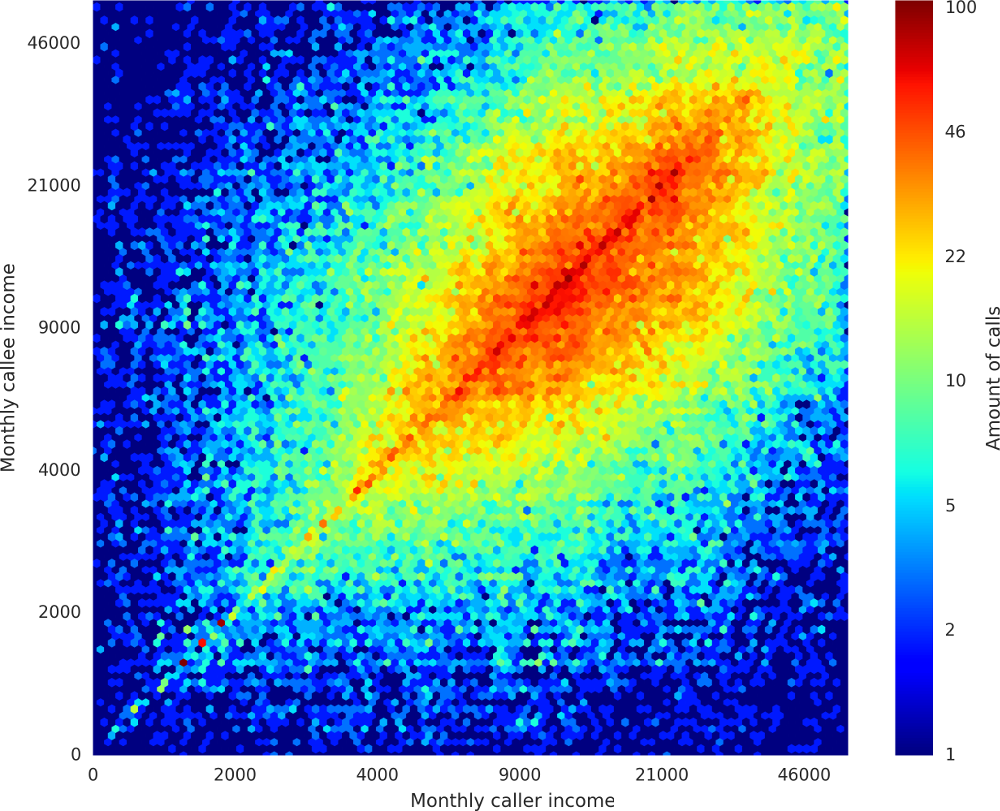
\includegraphics[width=.8\framewidth]{heatmap.png}
		\caption{Mapa de calor entre ingresos de usuarios de cada llamada.}
	\end{figure}
\end{frame}

\subsection{El Modelo Bayesiano}

\begin{frame}{El Modelo Bayesiano}
	La principal contribución de esta tesis es un modelo bayesiano de predicción de nivel de ingresos para los usuarios del grafo social y encontrar usuarios de altos ingresos.
\end{frame}

\begin{frame}{El Modelo Bayesiano}
	\begin{align*}
		H_1 &= \left\{ v \mid v \in V \wedge v_s \leq 6300 \right\} &\text{Usuarios de \emph{Bajos Ingresos}} \\
		H_2 &= \left\{ v \mid v \in V \wedge v_s >    6300 \right\} &\text{Usuarios de \emph{Altos Ingresos}}
	\end{align*}
\end{frame}

\begin{frame}{El Modelo Bayesiano}
	\begin{gather*}
		\begin{aligned}
			& \calls^{\low}_v = \sum_{\substack{e \in E \\ e_d = v \\ e_o \in H_1}}{e_c} + \sum_{\substack{e \in E \\ e_o = v \\ e_d \in H_1}}{e_c}
			& \calls^{\high}_v = \sum_{\substack{e \in E \\ e_d = v \\ e_o \in H_2}}{e_c} + \sum_{\substack{e \in E \\ e_o = v \\ e_d \in H_2}}{e_c} \\
			& \etime^{\low}_v = \sum_{\substack{e \in E \\ e_d = v \\ e_o \in H_1}}{e_t} + \sum_{\substack{e \in E \\ e_o = v \\ e_d \in H_1}}{e_t}
			& \etime^{\high}_v = \sum_{\substack{e \in E \\ e_d = v \\ e_o \in H_2}}{e_t} + \sum_{\substack{e \in E \\ e_o = v \\ e_d \in H_2}}{e_t} \\
			& \sms^{\low}_v = \sum_{\substack{e \in E \\ e_d = v \\ e_o \in H_1}}{e_s} + \sum_{\substack{e \in E \\ e_o = v \\ e_d \in H_1}}{e_s}
			& \sms^{\high}_v = \sum_{\substack{e \in E \\ e_d = v \\ e_o \in H_2}}{e_s} + \sum_{\substack{e \in E \\ e_o = v \\ e_d \in H_2}}{e_s}
		\end{aligned} \\
		\vspace{1em} \\
		\begin{aligned}
			\contacts^{\low}_v &= &\left| \left\{ e \in E \mid e_o = v \land e_d \in H_1 \right\} \cup \left\{ e \in E \mid e_d = v \land e_o \in H_1 \right\} \right| \\
			\contacts^{\high}_v &= &\left| \left\{ e \in E \mid e_o = v \land e_d \in H_2 \right\} \cup \left\{ e \in E \mid e_d = v \land e_o \in H_2 \right\} \right|
		\end{aligned}
	\end{gather*}
\end{frame}

\begin{frame}{El Modelo Bayesiano}
	\begin{equation*}
		\varpi \in \left\{ \calls, \etime, \sms, \contacts \right\}
	\end{equation*}
\end{frame}

\begin{frame}{El Modelo \sout{Bayesiano} Frecuentista}
	\onslide<1->{%
	\begin{equation*}
		p_v = P \left( v \in H_2 \right) = \frac{\varpi^{\high}_v}{\varpi^{\high}_v + \varpi^{low}_v}
	\end{equation*}
	}

	\onslide<2->{%
		Dados $a$ y $b$ donde
		
		\begin{gather*}
			\begin{aligned}
				&\calls^{\high}_a = 1   &\calls^{\low}_a = 0 \\
				&\calls^{\high}_b = 100 &\calls^{low}_b = 1
			\end{aligned} \\
			\vspace{1em} \\
			p_a > p_b
		\end{gather*}
	}

	\note{%
		Este modelo parece obviamente correcto, pero no modela la \emph{Incertidumbre} por la falta de información de dos usuarios
	}
\end{frame}

\begin{frame}{El Modelo Bayesiano}
	Se define una distribución Beta diferente para cada usuario $v \in V$.

	\begin{gather*}
		\Betasim_v \sim B \left( \varpi^{\high}_v + 1, \varpi^{\low} + 1 \right) \\
		\onslide<2-> {%
		P \left( \Betasim_v \leq x \right) = \frac{1}{B \left( \varpi^{\high} + 1, \varpi^{\low} + 1 \right)} \cdot \int^x_0 {t^{\varpi^{\high}_v} {\left( 1 - t \right)}^{\varpi^{\low}_v} dt}
		}
	\end{gather*}
	
	\onslide<3->{%
		Para medir la \emph{Incertidumbre}, se elige un cuántil arbitrario $\Theta \in \left[ 0, 1 \right]$ y se define
		\begin{align*}
			p_v &= Q \left( \Theta \right) \\
			&= \inf \left\{ x \in \left[ 0, 1 \right] \mid \Theta \leq F \left( x \right) \right\}
		\end{align*}

		Esta representa la \emph{posterior probability} de $p_v$ dados los datos.
	}
\end{frame}

\begin{frame}{El Modelo Bayesiano}
	\onslide<1->{%
		\begin{equation*}
			p_v = Q \left( \Theta \right)
		\end{equation*}
	}
	\onslide<1>{%
		Dados dos usuarios $v$ y $u$, $p_v > p_u$ implica que $v$ tiene mayor probabilidad de tener altos ingresos que $u$.

		Si $u$ tiene altos ingresos y $p_v > p_u$, $v$ tiene altos ingresos.
	}
	\onslide<2->{%
		\begin{gather*}
			\tau \in \left[ 0, 1 \right]  \\
			\vspace{1em} \\
			\begin{aligned}
				p_v \leq \tau &\implies v \in H_1 \\
				p_v >    \tau &\implies v \in H_2
			\end{aligned}
		\end{gather*}

		$\tau$ representa el umbral (threshold) que el algoritmo usa para separar usuarios de bajos y altos ingresos. Este valor puede usarse para incrementar o decrementar la precisión del modelo a cambio de recall.
	}
\end{frame}

\subsection{Evaluación del Modelo}

\begin{frame}{Evaluación del Modelo}
	\begin{itemize}
		\item $B$ Usuarios del banco.
		\pause{}
		\item $B_{\train}$ \emph{Training set} base.
		\item $B_{\test}$ \emph{Testing set} base.
			\begin{gather*}
				B = B_{\train} \cup B_{\test} \\
				\left| B_{\train} \right| = 0.8 \cdot \left|B\right| \qquad
				\left| B_{\test} \right| = 0.2 \cdot \left|B\right|
			\end{gather*}
		\pause{}
		\item $\hat{E}$ Usuarios con un algún vecino en el \emph{training set}.
		\item $\hat{B}_{\test}$ Usuarios del \emph{testing set} con algún vecino en el \emph{training set}.
			\begin{gather*}
				\hat{E} = \left\{ e \in E \mid e_o \in B_{\train} \lor e_d \in B_{\train} \right\} \\
				\hat{B}_{\test} = B_{\test} \cap \left( \hat{E}_o \cup \hat{E}_d \right)
			\end{gather*}
		\pause{}
		\item $\Upsilon$ Usuarios en $\hat{B}_{\test}$ con los labels balanceados.
			\begin{equation*}
				\left| \Upsilon_{\low} \right| = \left| \Upsilon_{\high} \right|
			\end{equation*}
	\end{itemize}
\end{frame}

\subsection{Optimizando $\Theta$}

\begin{frame}{Optimizando $\Theta$}
	Para medir la \emph{Incertidumbre}, se elige un cuántil arbitrario $\Theta \in \left[ 0, 1 \right]$ y se define
	\begin{align*}
		p_v &= Q \left( \Theta \right) \\
		&= \inf \left\{ x \in \left[ 0, 1 \right] \mid \Theta \leq F \left( x \right) \right\}
	\end{align*}

	Esta representa la \emph{posterior probability} de $p_v$ dados los datos.
\end{frame}

\begin{frame}{Optimizando $\Theta$}
	\begin{figure}
		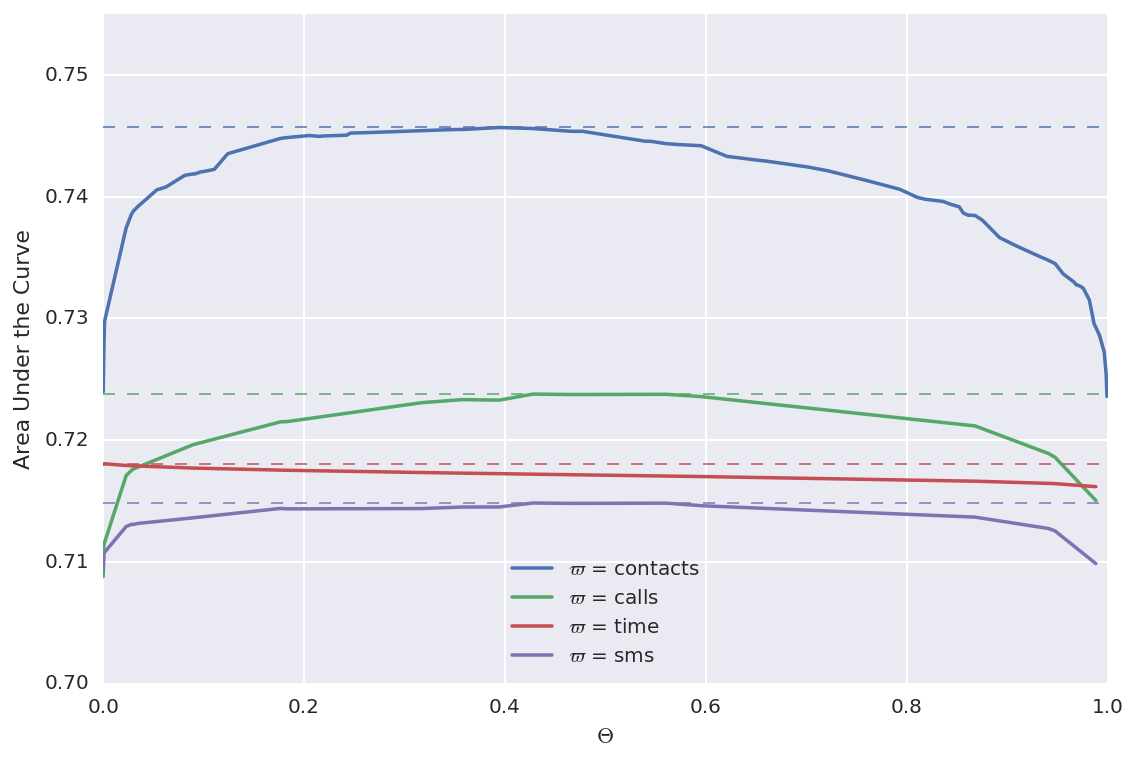
\includegraphics[height=.75\textheight]{theta.png}
		\caption{El \emph{área bajo la curva} del modelo bayesiano para diferentes $\varpi$ en base a $\Theta$.}
	\end{figure}
\end{frame}

\begin{frame}{Optimizando $\Theta$}
	\begin{table}
		\centering
		\begin{tabular}{l r r}
			\toprule
			\ct{$\varpi$}& \ct{$\Theta$ Óptimo} & \ct{AUC} \\
			\midrule
			contacts & \num{0.394} & \num{0.746} \\
			calls & \num{0.428} & \num{0.724} \\
			time & \num{0.001} & \num{0.718} \\
			sms & \num{0.428} & \num{0.715} \\
			\bottomrule
		\end{tabular}
		\caption{Resultados para $\Theta$ que maximizan el \emph{área bajo la curva}.}
	\end{table}
\end{frame}

\subsection{Optimizando $\tau$}

\begin{frame}{Optimizando $\tau$}
	\begin{itemize}
		\item Eligiendo un $\varpi$ y dado un $\Theta$, ya tenemos un buen modelo de predicción para $p_v$, la probabilidad de que $v$ sea un usuario de altos ingresos.
		\item $\tau$ representa el umbral (threshold) que el algoritmo usa para separar usuarios de bajos y altos ingresos.
			\begin{gather*}
				\begin{aligned}
					p_v \leq \tau &\implies v \in H_1 \\
					p_v >    \tau &\implies v \in H_2
				\end{aligned}
			\end{gather*}
		\item Para cada $\varpi$, se elige el $\tau$ que maximice la \emph{exactitud} (accuracy) del modelo.
	\end{itemize}
\end{frame}

\begin{frame}{Infiriendo por Cantidad de Llamadas}
		\begin{figure}
			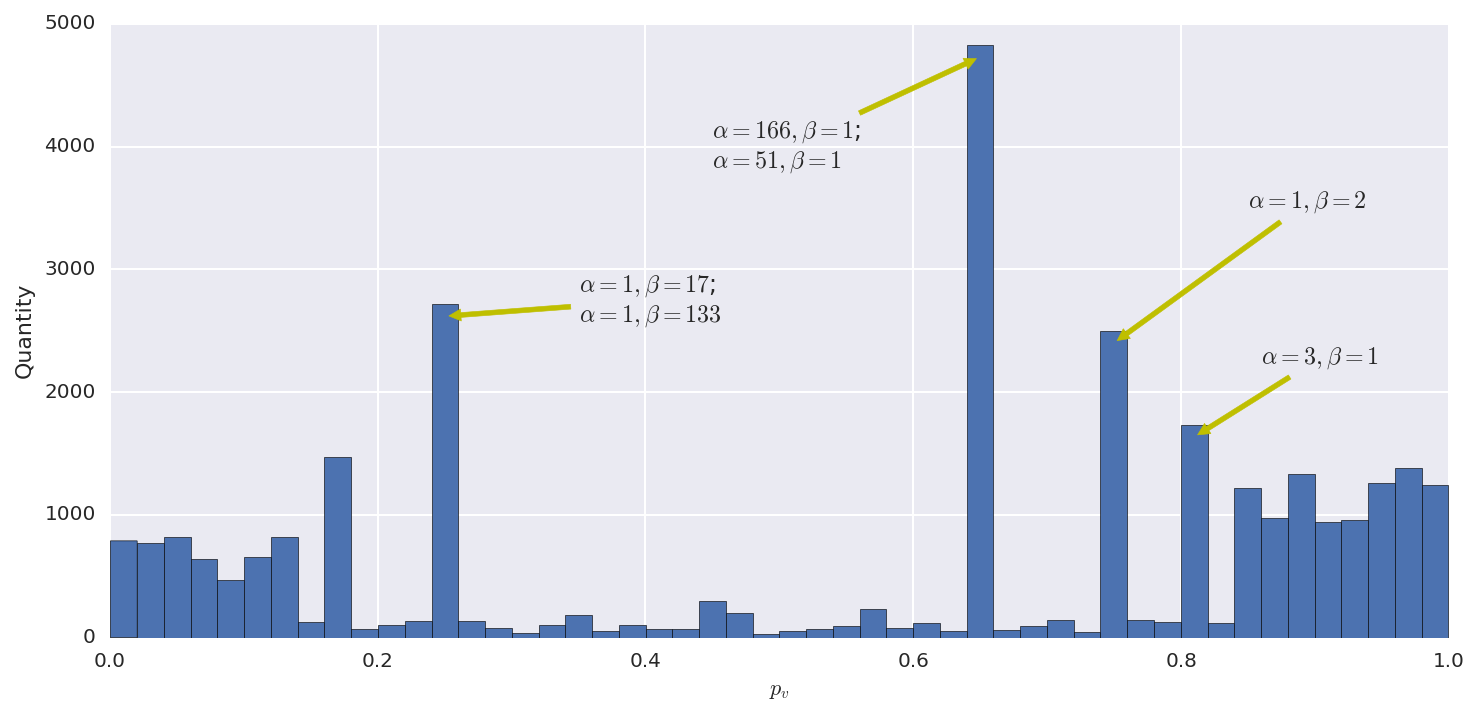
\includegraphics[width=\framewidth, height=.37\textheight, keepaspectratio]{bayes/hist_calls.png} \\
			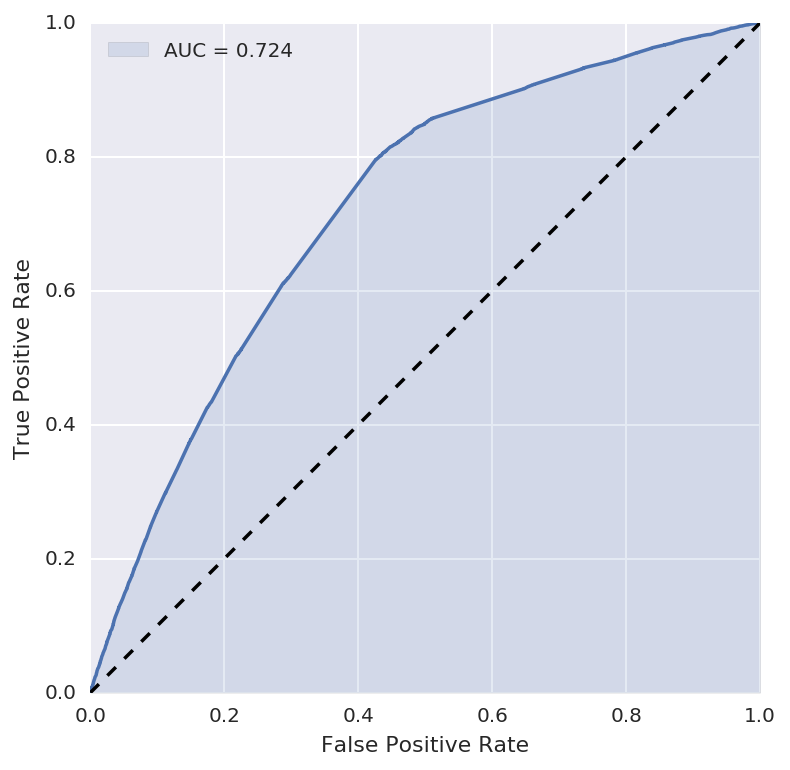
\includegraphics[width=.49\framewidth, height=.37\textheight, keepaspectratio]{bayes/roc_calls.png}
			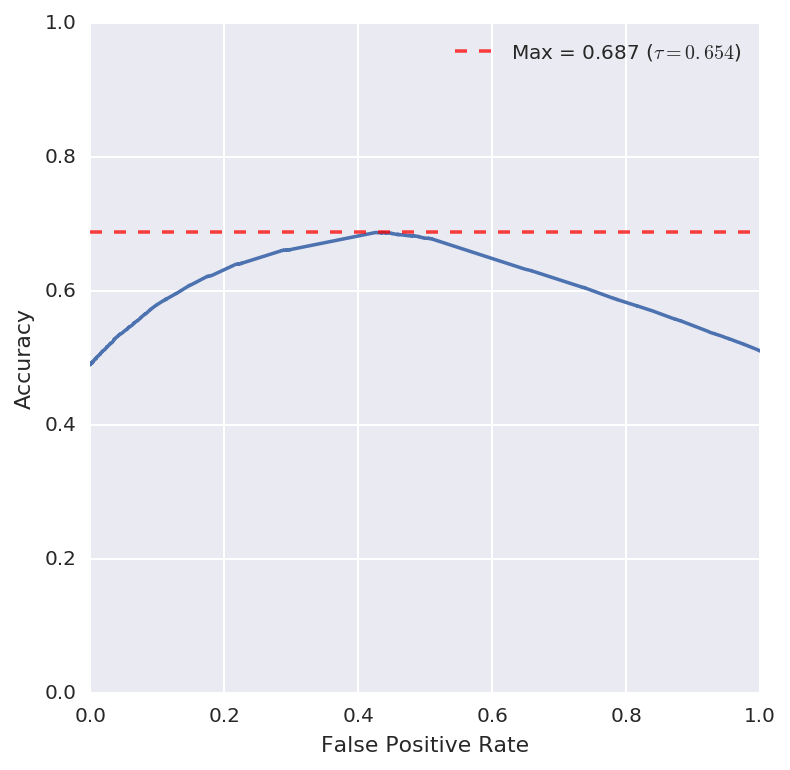
\includegraphics[width=.49\framewidth, height=.37\textheight, keepaspectratio]{bayes/accuracy_calls.png}
			\caption{Resultados del \emph{método bayesiano} usando cantidad de llamados. $\tau = 0.654$}
		\end{figure}

		\note{%
			\Cref{fig:bayes_calls} contains data about the predictor when $\varpi = \calls$ and the data is analyzed using $\Upsilon^{\calls}$ as \emph{Testing Set}. The \emph{Inverse Cumulative Distribution Function} contains a few peaks for users with a similar amount of calls.

			After analyzing the data, we find that the \emph{Area Under the Curve} using this method is of \num{0.724}, which is significantly higher than all the naïve and \emph{Machine Learning} methods that will be presented in the later \cref{sec:comparison}.

			Setting $\tau = 0.654$ maximizes the accuracy at $\Accuracy = 0.687$. Additionally, that value of $\tau$ results in $\Precision = 0.653$, $\Recall = 0.815$, $F_1 = 0.725$, and $F_4 = 0.804$.
			}
\end{frame}

\begin{frame}{Infiriendo por Tiempo Total de Llamadas}

	\begin{figure}
		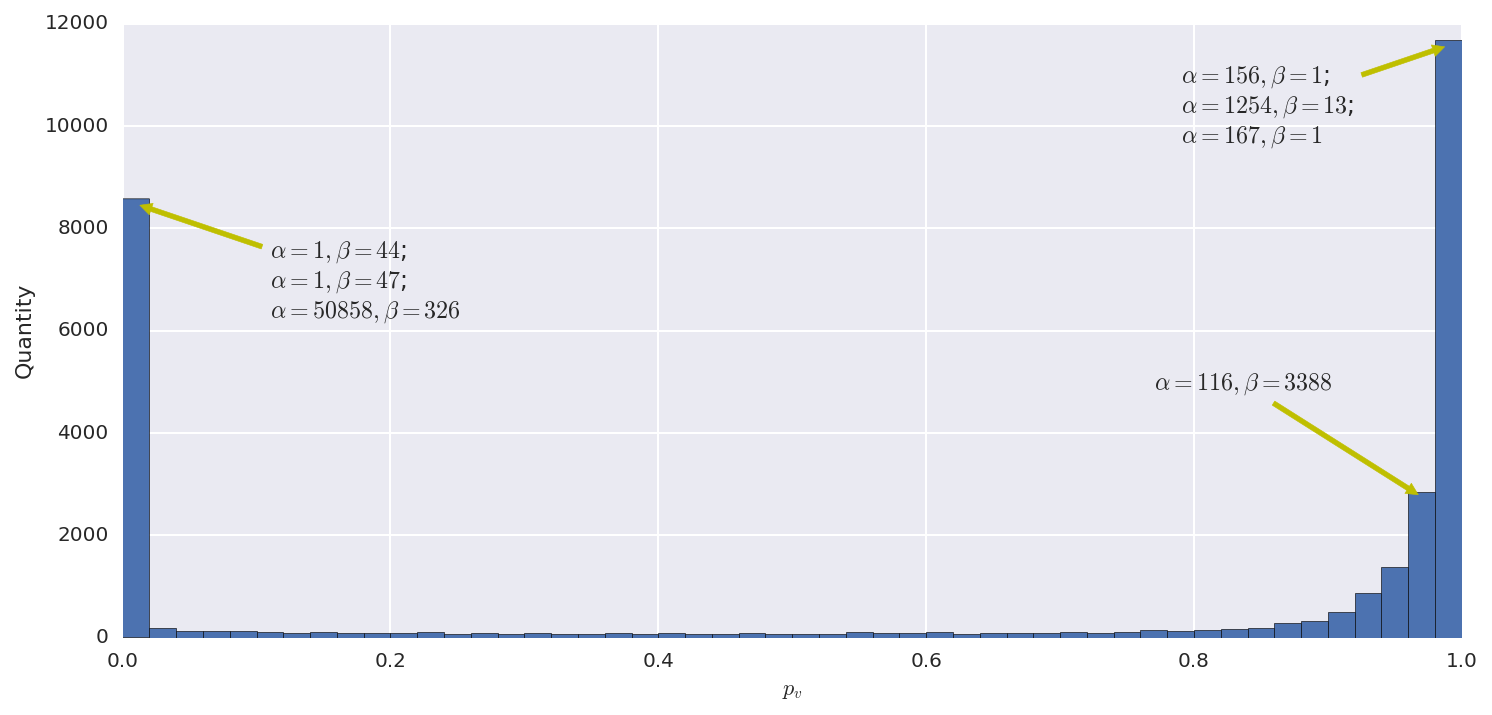
\includegraphics[width=\framewidth, height=.37\textheight, keepaspectratio]{bayes/hist_time.png} \\
		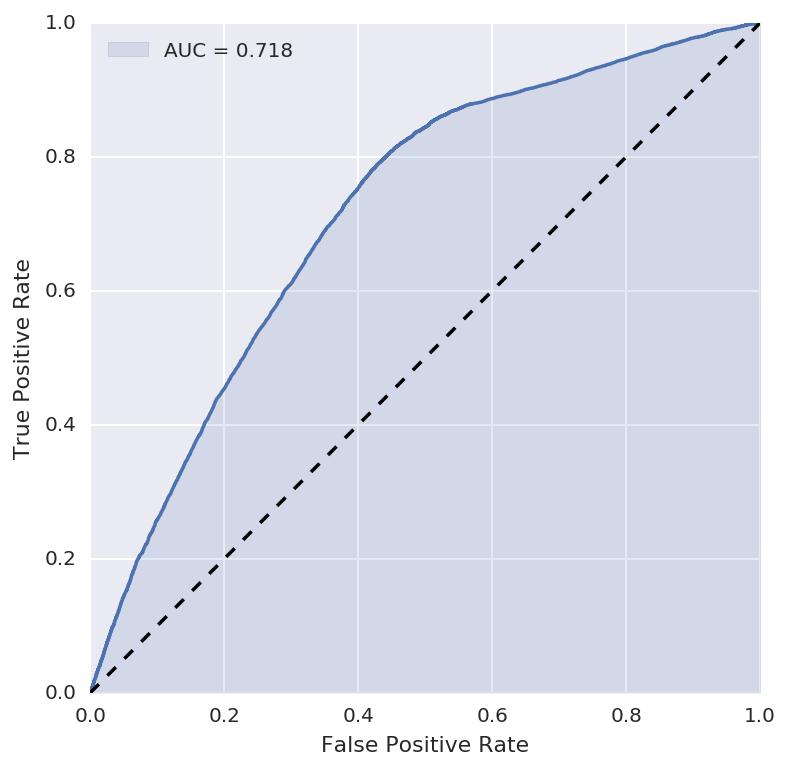
\includegraphics[width=.49\framewidth, height=.37\textheight, keepaspectratio]{bayes/roc_time.png}
		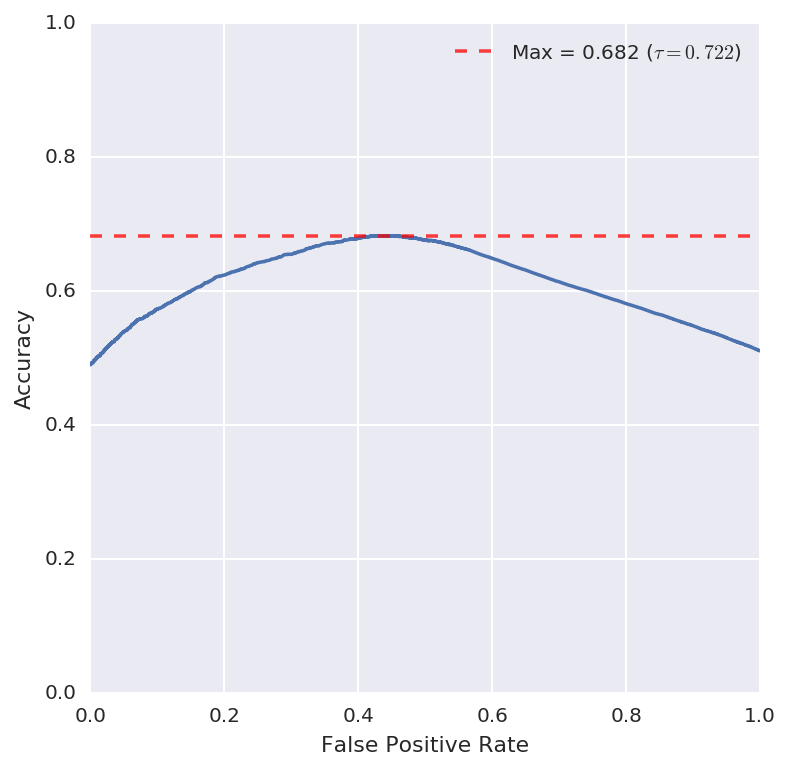
\includegraphics[width=.49\framewidth, height=.37\textheight, keepaspectratio]{bayes/accuracy_time.png}
		\caption{Resultados del \emph{método bayesiano} usando tiempo total de llamads. $\tau = 0.722$}
	\end{figure}

\note{%
	\Cref{fig:bayes_time} contains data about the predictor when $\varpi = \etime$ and the data is analyzed using $\Upsilon^{\calls}$ as \emph{Testing Set}, there are two big clusters of data at the edges; this is explained because the majority of users spend most of their time talking to either \emph{High Income} or \emph{Low Income} users.

	The \emph{Area Under the Curve} of this inference mechanism is $AUC = 0.718$, which is lower than the one for the calls in \cref{subsec:calls_infer}. The \emph{Accuracy Curve} is unsurprisingly similar to that one, and even the \emph{Accuracy} at $\tau = 0.722$ is the close. This is probably a result of the fact that there is an obvious correlation between total talking time and total calls.

	This $\tau$ also results in a predictor where $\Accuracy = 0.682$, $\Precision = 0.649$, $\Recall = 0.819$, $F_1 = 0.724$, and $F_4 = 0.807$.
}

\end{frame}

\begin{frame}{Infiriendo por Cantidad Total de Mensajes de Texto}

	\begin{figure}
		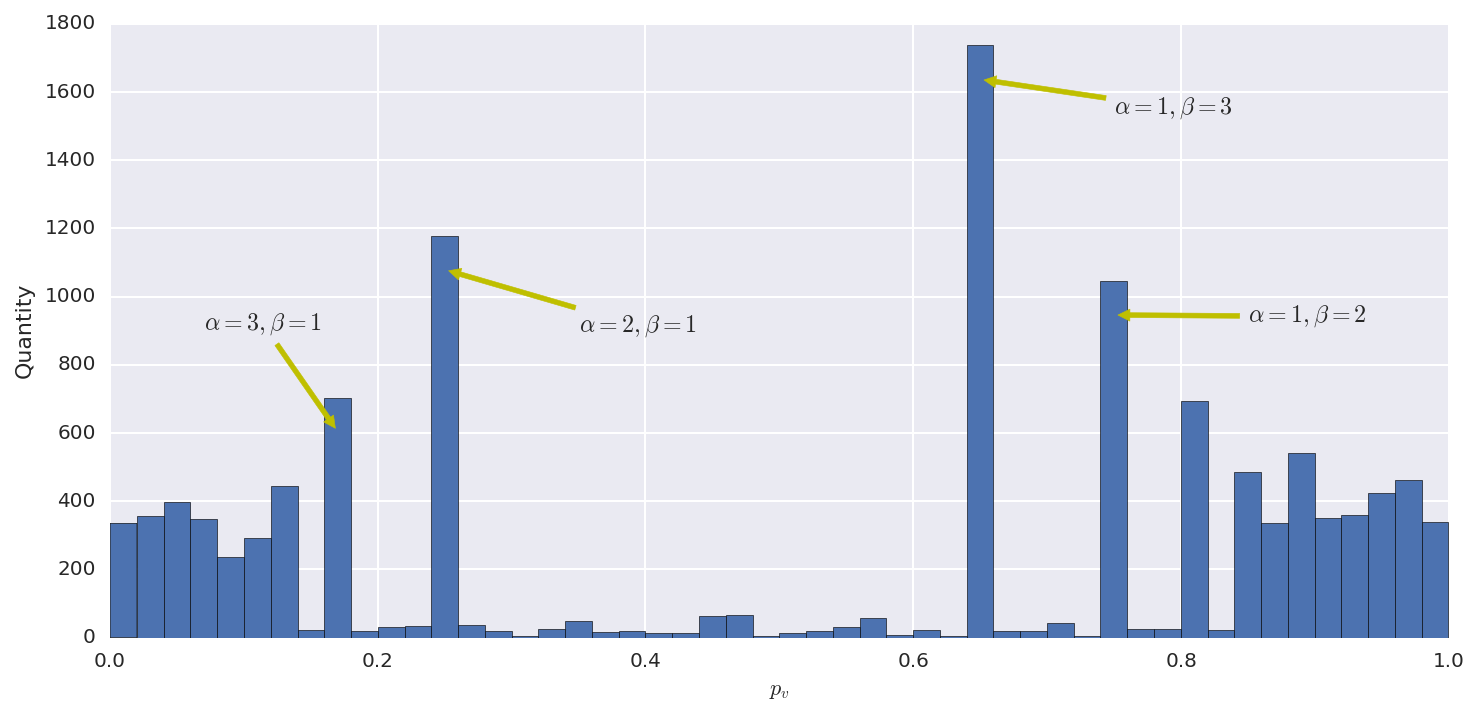
\includegraphics[width=\framewidth, height=.37\textheight, keepaspectratio]{bayes/hist_sms.png} \\
		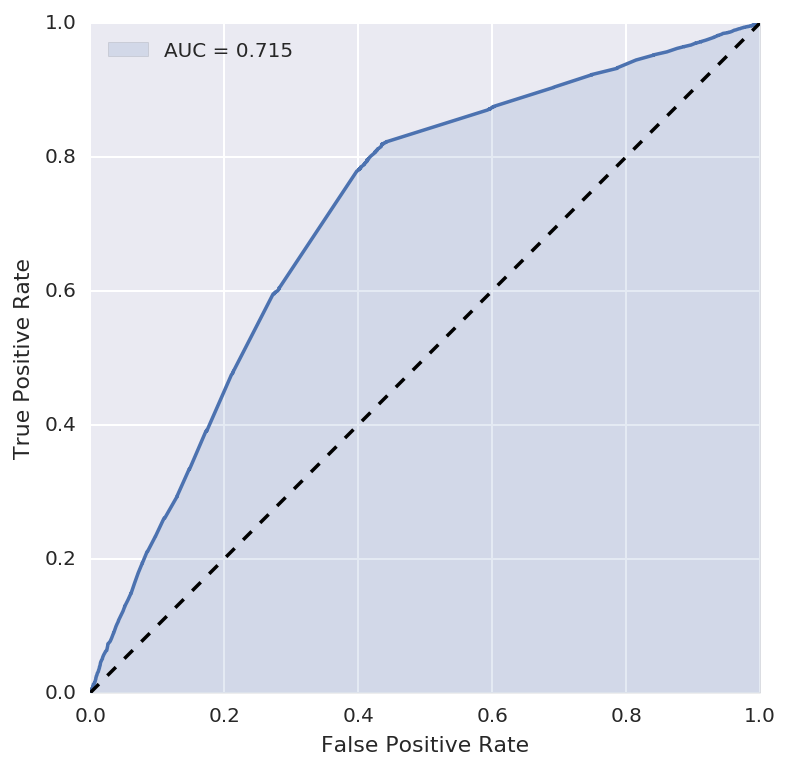
\includegraphics[width=.49\framewidth, height=.37\textheight, keepaspectratio]{bayes/roc_sms.png}
		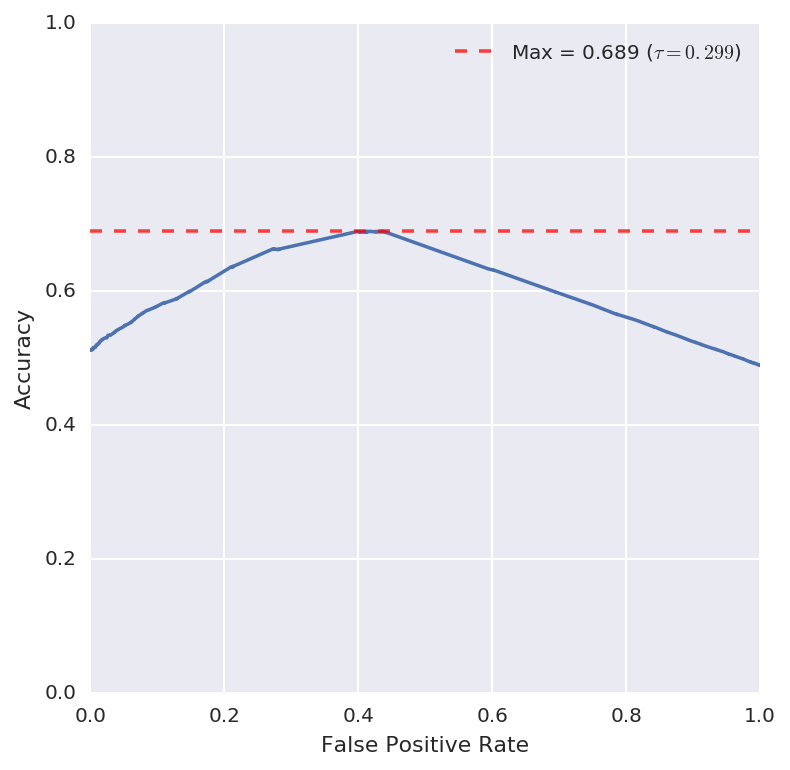
\includegraphics[width=.49\framewidth, height=.37\textheight, keepaspectratio]{bayes/accuracy_sms.png}
	\caption{Resultados del \emph{método bayesiano} usando cantidad total de mensajes de texto. $\tau = 0.299$}
	\end{figure}

	\note{%
		\Cref{fig:bayes_sms} shows the distributions when $\varpi = \sms$. Since the total amount of SMS is much lower than the amount of calls, the peaks of the result of the \emph{Inverse Cumulative Functions} of the \emph{Beta Distribution} applied on $\Upsilon^{\sms}$ that happen with the majority of users that have few of both are located closer to the center than in \cref{subsec:calls_infer,subsec:time_infer}. This makes some interesting cases if $\varpi = \sms$ is chosen, since the distribution is different than in the other cases.

		In particular, this gives an $AUC = 0.715$, which is lower than both in the case of \emph{Calls} and \emph{Time}. Interestingly, the maximum \emph{Accuracy} at $\tau = 0.299$ is slightly higher than both of the other cases; this is probably a side-effect of the fact that $\left| \Upsilon^{\sms} \right| < \left| \Upsilon^{\calls} \right|$.

		Additionally, $\Precision = 0.696$, $\Recall = 0.186$, $F_1 = 0.293$, and $F_4 = 0.194$.
	}

\end{frame}

\begin{frame}{Infiriendo por Cantidad de Contactos}

	\begin{figure}
		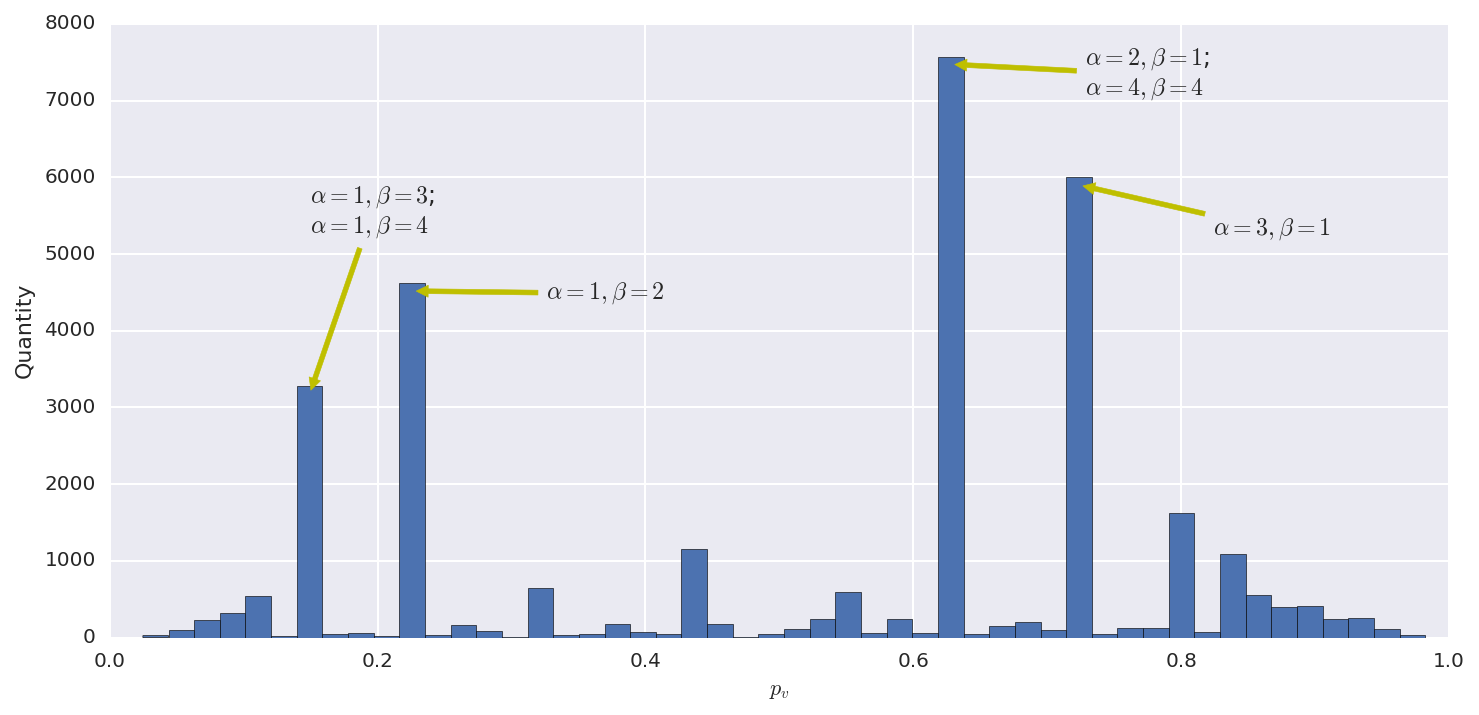
\includegraphics[width=\framewidth, height=.37\textheight, keepaspectratio]{bayes/hist_contacts.png} \\
		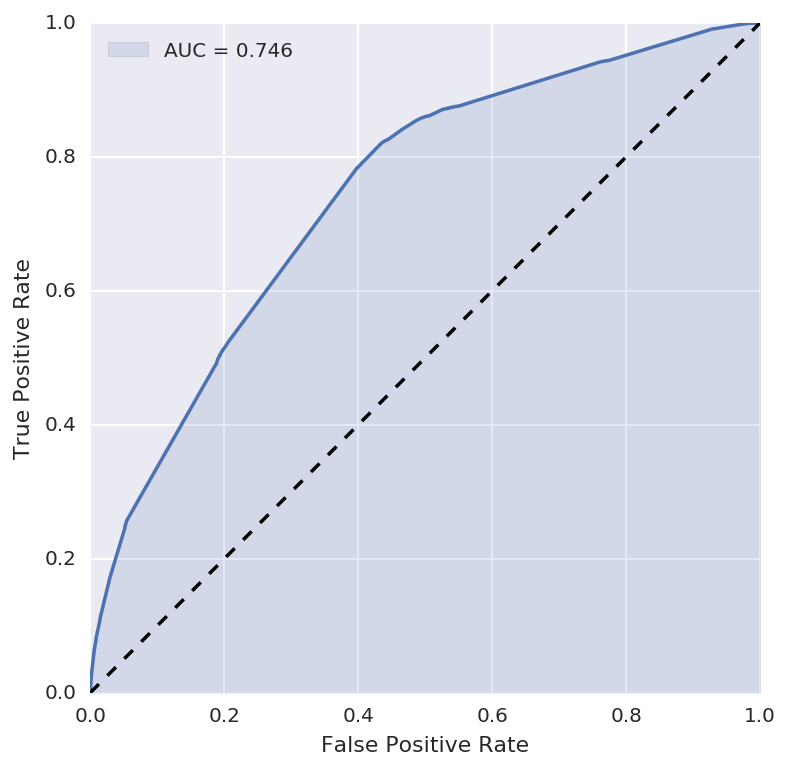
\includegraphics[width=.49\framewidth, height=.37\textheight, keepaspectratio]{bayes/roc_contacts.png}
		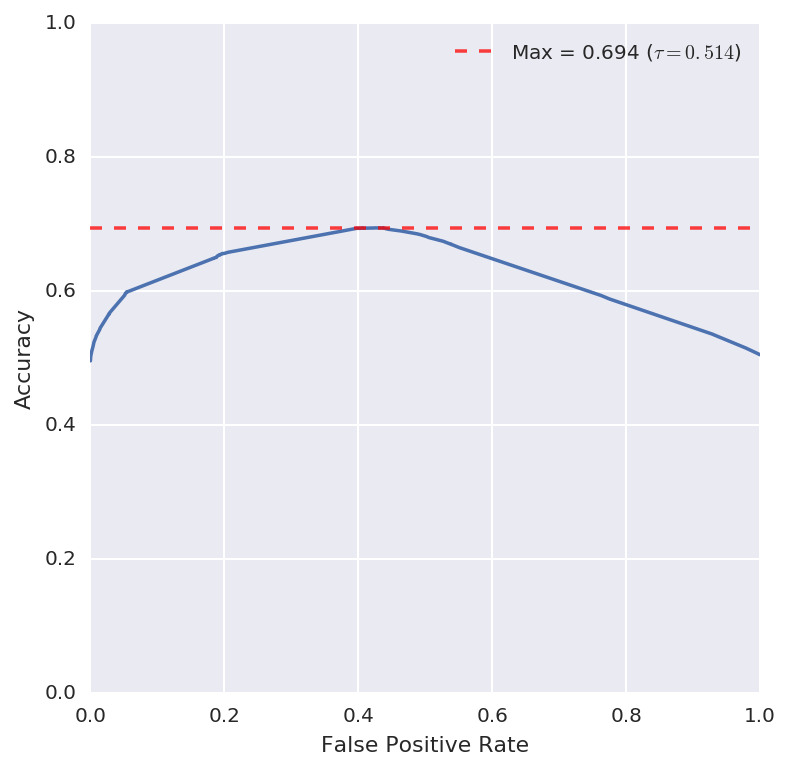
\includegraphics[width=.49\framewidth, height=.37\textheight, keepaspectratio]{bayes/accuracy_contacts.png}

		\caption{Resultados del \emph{método bayesiano} usando el grado de cada usuario. $\tau = 0.514$}
	\end{figure}

	\note{%
		\Cref{fig:bayes_contacts} shows the distributions when $\varpi = \contacts$, where it is possible to get a pattern similar to the one shown in \cref{subsec:sms_infer} when $\varpi = \sms$, where the majority of users have relatively few contacts and the peaks in the histogram. Additionally, since the total amount of contacts is exponentially distributed (as shown in \cref{fig:outcontacts_dist}), and people with \emph{High Income} tend to have more contacts in general, there peaks are clustered in areas with low $p_v$ (where the majority of calls are made to \emph{Low Income} users), near the middle (where the calls are mostly equally distributed), but not at high $p_v$; this last section would belong to the few users with many calls to \emph{High Income} users.

		Using this method it is possible to find that $AUC = 0.746$, which is higher than all the other methods presented in \cref{subsec:algorithm_performance}. Additionally, when selecting $\tau = 0.514$, $\Accuracy = 0.694$ which is higher than the maximum \emph{Accuracy} in all other methods. These metrics, combined with the fact that $\Upsilon$ contains every user in the \emph{Testing Set}, result in the fact that $\varpi = \contacts$ is unambiguously the best way to classify the data for the algorithm. Additionally, $\Precision = 0.556$, $\Recall = 0.792$, $F_1 = 0.723$, and $F_4 = 0.783$.
	}

\end{frame}

\subsection{Resultados Finales}

\begin{frame}{Resultados Finales}
	\begin{table}
		\begin{tabular}{l r r r r r r r r}
			\toprule
			$\varpi$ & \ct{$\Theta$} & \ct{$\tau$} & \ct{Acc.} & \ct{Prec.} & \ct{Rec.} & \ct{AUC} & \ct{F\textsubscript{1}} & \ct{F\textsubscript{4}} \\
			\midrule
			calls    & 0.428 & 0.654 & 0.686 & 0.654 & 0.816 & 0.724 & 0.726 & 0.804 \\
			time     & 0.001 & 0.722 & 0.681 & 0.652 & 0.806 & 0.718 & 0.721 & 0.795 \\
			sms      & 0.428 & 0.299 & 0.688 & 0.648 & 0.789 & 0.715 & 0.712 & 0.779 \\
			contacts & 0.394 & 0.514 & 0.693 & 0.665 & 0.792 & 0.746 & 0.723 & 0.783 \\
			\bottomrule
		\end{tabular}
		\caption{Metrics for the Bayesian algorithm using every user in $\Upsilon$}
	\end{table}

	\pause{}
	Las mejores métricas del algoritmo se van para estos hiperparámetros.
	\begin{align*}
		\varpi &= \contacts \\
		\Theta &= 0.394 \\
		\tau &= 0.514
	\end{align*}
\end{frame}

\section{Otros Modelos Basados en Aprendizaje Automático}

\subsection{Introducción}

\begin{frame}{Otros Modelos Basados en Aprendizaje Automático}
	Esta tesis presenta otros métodos basados en prácticas más comunes del aprendizaje automático. El problema a resolver sigue siendo el mismo.

	\begin{block}{}
		Dado un \emph{grafo social} $G = \left< V, E \right>$, buscar cuáles usuarios $v \in V$ tienen bajos ingresos [$v \in H_1$] y cuáles tienen altos ingresos [$v \in H_2$].
	\end{block}

\end{frame}

\subsection{Selección Aleatoria}

\begin{frame}{Selección Aleatoria}
	El método de selección aleatoria simplemente elige una categoría al azar.

	\begin{align*}
		P \left( v \in H_1 \right) &= \sfrac{1}{2} \\
		P \left( v \in H_2 \right) &= \sfrac{1}{2}
	\end{align*}
\end{frame}

\subsection{Votación Mayoritaria}
\begin{frame}{Votación Mayoritaria}
	El método de votación mayoritaria elige la categoría de cada usuario como la categoría a la que pertenecen la mayoría de sus contactos. En caso de empate, se elige una categoría al azar.

	\begin{equation*}
		P \left( v \in H_1 \right) =
		\begin{cases}
			0            & \text{si} \ \contacts^{\low}_{v} < \contacts^{\high}_{v} \\
			\sfrac{1}{2} & \text{si} \ \contacts^{\low}_{v} = \contacts^{\high}_{v} \\
			1            & \text{si} \ \contacts^{\low}_{v} > \contacts^{\high}_{v}
		\end{cases}
	\end{equation*}
\end{frame}

\subsection{Métodos de Extracción de Features}
\begin{frame}{Métodos de Extracción de Features en un Grafo}
	A continuación se presentan 6 métodos de extracción de features para el \emph{grafo social} $G$.
	\begin{itemize}
		\item Los métodos $\ego_{\left\{0, 1, 2\right\}}$, que usan datos sobre las aristas adyacentes a $n$ niveles del \emph{ego network} de cada nodo.
		\item Los métodos $\cat_{\left\{0, 1, 2\right\}}$, que separan estos datos en diferentes categorías dependiendo del nivel socioeconómico de cada vecino.
	\end{itemize}

	\begin{figure}
		\resizebox{!}{.4\textheight}{%
			\framebox{%
				
\begin{tikzpicture}[>=latex,line join=bevel,]
%%
\begin{scope}
  \pgfsetstrokecolor{black}
  \definecolor{strokecol}{rgb}{1.0,1.0,1.0};
  \pgfsetstrokecolor{strokecol}
  \definecolor{fillcol}{rgb}{1.0,1.0,1.0};
  \pgfsetfillcolor{fillcol}
  \filldraw (0.0bp,0.0bp) -- (0.0bp,168.0bp) -- (90.0bp,168.0bp) -- (90.0bp,0.0bp) -- cycle;
\end{scope}
\begin{scope}
  \pgfsetstrokecolor{black}
  \definecolor{strokecol}{rgb}{1.0,1.0,1.0};
  \pgfsetstrokecolor{strokecol}
  \definecolor{fillcol}{rgb}{1.0,1.0,1.0};
  \pgfsetfillcolor{fillcol}
  \filldraw (0.0bp,0.0bp) -- (0.0bp,168.0bp) -- (90.0bp,168.0bp) -- (90.0bp,0.0bp) -- cycle;
\end{scope}
\begin{scope}
  \pgfsetstrokecolor{black}
  \definecolor{strokecol}{rgb}{1.0,1.0,1.0};
  \pgfsetstrokecolor{strokecol}
  \definecolor{fillcol}{rgb}{1.0,1.0,1.0};
  \pgfsetfillcolor{fillcol}
  \filldraw (0.0bp,0.0bp) -- (0.0bp,168.0bp) -- (90.0bp,168.0bp) -- (90.0bp,0.0bp) -- cycle;
\end{scope}
\begin{scope}
  \pgfsetstrokecolor{black}
  \definecolor{strokecol}{rgb}{1.0,1.0,1.0};
  \pgfsetstrokecolor{strokecol}
  \definecolor{fillcol}{rgb}{1.0,1.0,1.0};
  \pgfsetfillcolor{fillcol}
  \filldraw (0.0bp,0.0bp) -- (0.0bp,168.0bp) -- (90.0bp,168.0bp) -- (90.0bp,0.0bp) -- cycle;
\end{scope}
  \node (d0p) at (72.0bp,106.0bp) [draw,circle] {$cat_0$};
  \node (d1p) at (72.0bp,62.0bp) [draw,circle] {$cat_1$};
  \node (d2p) at (72.0bp,18.0bp) [draw,circle] {$cat_2$};
  \coordinate (inv2) at (18.0bp,18.0bp);
  \coordinate (inv0) at (72.0bp,150.0bp);
  \node (0) at (18.0bp,150.0bp) [draw,circle] {$ego_0$};
  \node (1) at (18.0bp,106.0bp) [draw,circle] {$ego_1$};
  \node (2) at (18.0bp,62.0bp) [draw,circle] {$ego_2$};
  \definecolor{strokecolor}{rgb}{0.0,0.25,0.0};
  \draw [strokecolor,-stealth'] (2) ..controls (37.602bp,46.028bp) and (43.91bp,40.888bp)  .. (d2p);
  \definecolor{strokecolor}{rgb}{0.0,0.0,0.25};
  \draw [strokecolor,-stealth'] (d1p) ..controls (72.0bp,43.69bp) and (72.0bp,43.53bp)  .. (d2p);
  \definecolor{strokecolor}{rgb}{0.0,0.25,0.0};
  \draw [strokecolor,-stealth'] (1) ..controls (37.602bp,90.028bp) and (43.91bp,84.888bp)  .. (d1p);
  \definecolor{strokecolor}{rgb}{0.0,0.25,0.0};
  \draw [strokecolor,-stealth'] (0) ..controls (37.602bp,134.03bp) and (43.91bp,128.89bp)  .. (d0p);
  \definecolor{strokecolor}{rgb}{0.0,0.0,0.25};
  \draw [strokecolor,-stealth'] (d0p) ..controls (72.0bp,87.69bp) and (72.0bp,87.53bp)  .. (d1p);
  \definecolor{strokecolor}{rgb}{0.0,0.0,0.25};
  \draw [strokecolor,-stealth'] (0) ..controls (18.0bp,131.69bp) and (18.0bp,131.53bp)  .. (1);
  \definecolor{strokecolor}{rgb}{0.0,0.0,0.25};
  \draw [strokecolor,-stealth'] (1) ..controls (18.0bp,87.69bp) and (18.0bp,87.53bp)  .. (2);
%
\end{tikzpicture}


			}
		}
		\caption{Relaciones entre los métodos de extracción de features.}
	\end{figure}
\end{frame}

\subsection{User Data --- Método $\ego_0$}
\begin{frame}{User Data --- Método $\ego_0$}
	Este método acumula diferentes features de las aristas de cada usuario.

	\begin{equation*}
		\begin{gathered}
			\begin{aligned}
				\incalls_v &= \sum_{\substack{e \in E \\ e_d = v}} \calls_e &
				\outcalls_v &= \sum_{\substack{e \in E \\ e_o = v}} \calls_e \\
				\intime_v &= \sum_{\substack{e \in E \\ e_d = v}} \etime_e &
				\outtime_v &= \sum_{\substack{e \in E \\ e_o = v}} \etime_e \\
				\insms_v &= \sum_{\substack{e \in E \\ e_d = v}} \sms_e &
				\outsms_v &= \sum_{\substack{e \in E \\ e_o = v}} \sms_e \\
			\end{aligned} \\
			\begin{aligned}
				\incontacts_v &= \left| \left\{ e \in E \mid e_d = v \right\} \right| \\
				\outcontacts_v &= \left| \left\{ e \in E \mid e_o = v \right\} \right|
			\end{aligned}
		\end{gathered}
	\end{equation*}

	\note{%
		Donde $E$ es el conjunto de aristas del \emph{grafo social}, y $\calls_e$, $\etime_e$, y $\sms_e$ son la cantidad de llamadas, el tiempo total de charla, y la cantidad de SMS en la arista $e$.
	}
\end{frame}

\subsection{Categorical User Data --- Método $\cat_0$}
\begin{frame}{Categorical User Data --- Método $\cat_0$}
	Los nodos $\Upsilon \subseteq V$ en los que se va a evaluar este métodos contiene información bancaria de los usuarios. 

	Esto permite crear features con los siguientes nombres.


	\begin{equation*}
		\begin{Bmatrix} \text{in} \\ \text{out} \end{Bmatrix}
		\times
		\begin{Bmatrix} \text{calls} \\ \text{time} \\ \text{sms} \\ \text{contacts} \end{Bmatrix}
		\times
		\begin{Bmatrix} \text{low} \\ \text{high} \end{Bmatrix}
	\end{equation*}

	Todos estos features se general de una manera similar a la siguiente ecuación.

	\begin{align*}
		\operatorname{incallslow}_v  = \sum_{\substack{e \in E \\ e_d \in H_1 \\ e_o = v}} &\calls_e &
		\operatorname{incallshigh}_v = \sum_{\substack{e \in E \\ e_d \in H_2 \\ e_o = v}} &\calls_e
	\end{align*}
\end{frame}


\subsection{Higher Order User Data --- Método $\ego_n$}
\begin{frame}{Higher Order User Data --- Método $\ego_n$}
	El \emph{Ego Network de Orden $n$} de un nodo $v$ contiene el nodo $v$, y todos los nodos y las aristas a los que tienen distancia $\leq n$ a $v$.

\begin{figure}
	\framebox{%
		
\begin{tikzpicture}[>=latex,line join=bevel,]
%%
\node (b4) at (58.264bp,80.697bp) [draw,ellipse] {};
  \node (b5) at (107.65bp,46.247bp) [draw,ellipse] {};
  \node (b6) at (134.09bp,46.247bp) [draw,ellipse] {};
  \node (b7) at (183.48bp,80.697bp) [draw,ellipse] {};
  \node (b0) at (183.48bp,124.78bp) [draw,ellipse] {};
  \node (b1) at (158.52bp,150.63bp) [draw,ellipse] {};
  \node (b2) at (107.65bp,159.23bp) [draw,ellipse] {};
  \node (b3) at (64.526bp,134.74bp) [draw,ellipse] {};
  \node (c11) at (64.398bp,30.901bp) [draw,ellipse] {};
  \node (c10) at (36.354bp,54.739bp) [draw,ellipse] {};
  \node (a1) at (92.698bp,86.739bp) [draw,ellipse] {};
  \node (a0) at (133.84bp,129.35bp) [draw,ellipse] {};
  \node (c9) at (21.176bp,85.884bp) [draw,ellipse] {};
  \node (a2) at (139.69bp,78.794bp) [draw,ellipse] {};
  \node (c3) at (140.7bp,18.0bp) [draw,ellipse] {};
  \node (c2) at (220.56bp,85.884bp) [draw,ellipse] {};
  \node (c1) at (205.39bp,54.739bp) [draw,ellipse] {};
  \node (c0) at (220.56bp,119.6bp) [draw,ellipse] {};
  \node (c7) at (205.39bp,150.74bp) [draw,ellipse] {};
  \node (c6) at (64.398bp,174.58bp) [draw,ellipse] {};
  \node (c5) at (101.04bp,187.48bp) [draw,ellipse] {};
  \node (c4) at (140.7bp,187.48bp) [draw,ellipse] {};
  \node (a3) at (152.17bp,91.719bp) [draw,ellipse] {};
  \node (c8) at (21.176bp,119.6bp) [draw,ellipse] {};
  \node (v) at (120.87bp,102.74bp) [draw,fill=gray,ellipse] {v};
  \draw [red,] (v) ..controls (135.03bp,84.728bp) and (135.11bp,84.621bp)  .. (a2);
  \draw [ForestGreen,] (b6) ..controls (138.26bp,28.429bp) and (138.28bp,28.341bp)  .. (c3);
  \draw [blue,] (a1) ..controls (80.328bp,107.82bp) and (76.815bp,113.8bp)  .. (b3);
  \draw [ForestGreen,] (b7) ..controls (166.4bp,55.662bp) and (157.67bp,42.867bp)  .. (c3);
  \draw [blue,] (a0) ..controls (121.21bp,143.76bp) and (120.45bp,144.63bp)  .. (b2);
  \draw [ForestGreen,] (b2) ..controls (87.533bp,166.37bp) and (84.387bp,167.49bp)  .. (c6);
  \draw [ForestGreen,] (b4) ..controls (41.841bp,97.922bp) and (37.585bp,102.39bp)  .. (c8);
  \draw [red,] (v) ..controls (142.36bp,95.175bp) and (142.44bp,95.145bp)  .. (a3);
  \draw [ForestGreen,] (b7) ..controls (199.9bp,97.922bp) and (204.16bp,102.39bp)  .. (c0);
  \draw [blue,] (a0) ..controls (147.71bp,141.31bp) and (147.8bp,141.39bp)  .. (b1);
  \draw [ForestGreen,] (b0) ..controls (195.28bp,138.77bp) and (195.36bp,138.87bp)  .. (c7);
  \draw [ForestGreen,] (b4) ..controls (61.028bp,58.262bp) and (61.616bp,53.483bp)  .. (c11);
  \draw [ForestGreen,] (b2) ..controls (103.48bp,177.05bp) and (103.46bp,177.14bp)  .. (c5);
  \draw [blue,] (a1) ..controls (74.544bp,83.554bp) and (74.414bp,83.531bp)  .. (b4);
  \draw [red,] (v) ..controls (130.88bp,123.29bp) and (130.94bp,123.4bp)  .. (a0);
  \draw [ForestGreen,] (b7) ..controls (195.28bp,66.71bp) and (195.36bp,66.613bp)  .. (c1);
  \draw [blue,] (a0) ..controls (156.36bp,127.28bp) and (160.96bp,126.85bp)  .. (b0);
  \draw [ForestGreen,] (b4) ..controls (46.458bp,66.71bp) and (46.377bp,66.613bp)  .. (c10);
  \draw [blue,] (a3) ..controls (169.4bp,85.652bp) and (169.52bp,85.612bp)  .. (b7);
  \draw [ForestGreen,] (b5) ..controls (87.533bp,39.109bp) and (84.387bp,37.993bp)  .. (c11);
  \draw [ForestGreen,] (b2) ..controls (123.17bp,172.5bp) and (124.91bp,173.98bp)  .. (c4);
  \draw [blue,] (a1) ..controls (99.753bp,67.634bp) and (100.57bp,65.415bp)  .. (b5);
  \draw [blue,] (a2) ..controls (136.61bp,60.878bp) and (136.59bp,60.759bp)  .. (b6);
  \draw [red,] (v) ..controls (100.85bp,91.371bp) and (100.71bp,91.289bp)  .. (a1);
  \draw [blue,] (a1) ..controls (110.72bp,69.108bp) and (116.32bp,63.636bp)  .. (b6);
  \draw [blue,] (a1) ..controls (98.712bp,115.9bp) and (101.69bp,130.32bp)  .. (b2);
  \draw [ForestGreen,] (b7) ..controls (201.88bp,83.271bp) and (202.17bp,83.312bp)  .. (c2);
  \draw [ForestGreen,] (b4) ..controls (39.861bp,83.271bp) and (39.566bp,83.312bp)  .. (c9);
  \draw [ForestGreen,] (b0) ..controls (201.88bp,122.21bp) and (202.17bp,122.17bp)  .. (c0);
%
\end{tikzpicture}


	}
	\caption{Los ejes que se usan al calcular el método $\ego_2$ de un nodo $v$. Las aristas \textcolor{red}{rojas} son las aristas usadas en $\ego_{n \geq 0}$, las \textcolor{blue}{azules} las usadas en $\ego_{n \geq 1}$, y las \textcolor{ForestGreen}{verdes} los que se usan en $\ego_{n \geq 2}$.}
\end{figure}
\end{frame}

\begin{frame}{Higher Order User Data --- Método $\ego_n$}
	Se extienden los features del método $\ego_0$ con datos del \emph{Ego Network de Orden $n$} de $v$.

	\begin{align*}
		\incalls^n_v  = \meight\sum_{\substack{e \in E \\ d(e_o, v) = n \\ d(e_d, v) = n + 1}}\meight&\calls_e &
		\outcalls^n_v = \meight\sum_{\substack{e \in E \\ d(e_d, v) = n \\ d(e_o, v) = n + 1}}\meight &\calls_e
	\end{align*}
\end{frame}

\subsection{Categorical Higher Order User Data --- Método $\cat_n$}
\begin{frame}{Categorical Higher Order User Data --- Método $\cat_n$}
	Se extienden los features del método $\cat_0$ con datos del \emph{Ego Network de Orden $n$} de $v$, donde cada arista agrega diferentes valores para los vecinos de bajo y alto nivel socioeconómico.

	\begin{align*}
		\operatorname{incallslow}^n_v = \meight\sum_{\substack{e \in E \\ e_d \in H_1 \\ d \left( e_o, v \right) = n \\ d \left( e_d, v \right) = n + 1}}\meight \calls_e &\quad
		\operatorname{incallshigh}^n_v = \meight\sum_{\substack{e \in E \\ e_d \in H_2 \\ d \left( e_o, v \right) = n \\ d \left( e_d, v \right) = n + 1}}\meight \calls_e \\
		\vspace{1em} \\
		\operatorname{outcallslow}^n_v = \meight\sum_{\substack{e \in E \\ e_o \in H_1 \\ d \left( e_d, v \right) = n \\ d \left( e_o, v \right) = n + 1}}\meight \calls_e &\quad
		\operatorname{outcallshigh}^n_v = \meight\sum_{\substack{e \in E \\ e_o \in H_2 \\ d \left( e_d, v \right) = n \\ d \left( e_o, v \right) = n + 1}}\meight \calls_e \\
		\vspace{1em} \\
	\end{align*}
\end{frame}

\subsection{Métodos de Machine Learning}
\begin{frame}{Métodos de Machine Learning}
	Cada uno de estos conjuntos de features es entrenado usando uno de estos métodos de aprendizaje automático y grid search usando stratified 5-fold validation, y luego evaluado el resultado en $\Upsilon$.
	\begin{itemize}
		\item \emph{Regresión Lineal}, eligiendo el coeficiente regulador $C$ en incrementos exponenciales.
			\begin{equation*}
				C \in \left\{ 10^{-3}, 10^{-2}, 10^{-1}, 10^0, 10^1, 10^2, 10^3 \right\}
			\end{equation*}
		\item \emph{Random Forest}, con alguno de los siguientes hiperparámetros, donde $f$ es la cantidad de features para este método.
			\begin{align*}
				\operatorname{Criterion} &\in \left\{ \operatorname{Gini}, \operatorname{Entropy} \right\} \\
				\operatorname{Features} &\in \left\{ f, \sqrt{f}, \log_2{f} \right\} \\
				\operatorname{Replacement} &\in \left\{ \operatorname{True}, \operatorname{False} \right\}
			\end{align*}
	\end{itemize}
\end{frame}

\section{Resultados Finales}

\subsection{Resultados}
\begin{frame}{Resultados}
	El método bayesiano, los 2 métodos triviales, y los 2 métodos de aprendizaje automático aplicados a los 6 métodos de extracción de features se entrenaron con el mismo conjunto de datos y fueron evaluados en $\Upsilon$ en un server con las siguientes propiedades.

	\begin{itemize}
		\item Intel Xeon D-1540 con 2GHZ y 128GByte de RAM.\@  \\
		\item Numpy 1.12.1 \\
		\item Scipy 0.18.1 \\
		\item Padas 0.19.2 \\
		\item Scikit-learn 0.18
	\end{itemize}
\end{frame}

\begin{frame}{Resultados}
	\resizebox{\framewidth}{!}{%
		\begin{tabular}{l l r r r r r r r r}
			\toprule
			\ct{Modelo} & \ct{Features} & \ct{Acc.} & \ct{Prec.} & \ct{Rec.} & \ct{AUC} & \ct{F\textsubscript{1}} & \ct{F\textsubscript{4}} & \ct{t\textsubscript{fit}} & \ct{t\textsubscript{pred}} \\

			\midrule

			&&&&&&&&& \\
			\midrule

			\multicolumn{2}{l}{Aleatorio}
			& 0.499 & 0.499 & 0.500 & 0.499 & 0.500 & 0.500 & \ct{\NA} & \SI{0.005}{\second} \\

			\multicolumn{2}{l}{Mayoría}
			& 0.681 & 0.640 & 0.826 & 0.681 & 0.721 & 0.712 & \ct{\NA} & \SI{0.059}{\second} \\

			\midrule

			\multirow{6}{*}{LR}
			& $\ego_0$ & 0.536 & 0.531 & 0.625 & 0.536 & 0.574 & 0.619 & \SI{0.145}{\second}   & \SI{0.002}{\second} \\
			& $\ego_1$ & 0.535 & 0.525 & 0.730 & 0.535 & 0.611 & 0.714 & \SI{0.141}{\second}   & \SI{0.011}{\second} \\
			& $\ego_2$ & 0.568 & 0.578 & 0.525 & 0.569 & 0.550 & 0.528 & \SI{0.119}{\second}   & \SI{0.003}{\second} \\
			& $\cat_0$ & 0.686 & 0.655 & 0.785 & 0.686 & 0.714 & 0.776 & \SI{0.167}{\second}   & \SI{0.005}{\second} \\
			& $\cat_1$ & 0.693 & 0.665 & 0.780 & 0.693 & 0.718 & 0.772 & \SI{1.588}{\second}   & \SI{0.011}{\second} \\
			& $\cat_2$ & 0.693 & 0.670 & 0.764 & 0.692 & 0.714 & 0.758 & \SI{0.956}{\second}   & \SI{0.009}{\second} \\
			\midrule

			\multirow{6}{*}{RF}
			& $\ego_0$ & 0.548 & 0.548 & 0.550 & 0.548 & 0.549 & 0.550 & \SI{5.986}{\second}   & \SI{0.588}{\second} \\
			& $\ego_1$ & 0.582 & 0.583 & 0.577 & 0.582 & 0.580 & 0.577 & \SI{56.548}{\second}  & \SI{0.483}{\second} \\
			& $\ego_2$ & 0.576 & 0.577 & 0.580 & 0.576 & 0.579 & 0.580 & \SI{50.197}{\second}  & \SI{0.253}{\second} \\
			& $\cat_0$ & 0.671 & 0.665 & 0.690 & 0.671 & 0.677 & 0.688 & \SI{6.346}{\second}   & \SI{0.539}{\second} \\
			& $\cat_1$ & 0.714 & 0.713 & 0.716 & 0.714 & 0.714 & 0.716 & \SI{96.005}{\second}  & \SI{0.460}{\second} \\
			& $\cat_2$ & 0.709 & 0.710 & 0.711 & 0.709 & 0.711 & 0.711 & \SI{81.528}{\second}  & \SI{0.242}{\second} \\
			\bottomrule

		\end{tabular}
	}

	\note{%
		Con estos datos, se pueden sacar varias conclusiones.
		\begin{itemize}
			\item Como los datos no son lineales, los métodos basados en \emph{Random Forest} tienen mejores resultados que los basados en \emph{Regresión Lineal}. Esto es consistente con muchos experimentos similares, como los de Muchlinski et~al.~\footcite{muchlinski2016}~\footcite{logisticvsdecision}. \\
			\item El método basado en \emph{Random Forest} tiene mejores resultados cuando se agregan features nuevos, como en la diferencia entre $\ego_0$ y $\ego_1$. Interesantemente, la mayoría de las métricas presentan un decrecimiento cuando suben un nivel más a $\ego_2$, aunque este sea un superconjunto del anterior. Una posible razón es que los nuevos features traen ruido al entrenamiento del \emph{Random Forest}. \\
			\item La mayor mejora de los métodos basados en aprendizaje automático es agregando labels que dependen del nivel socioeconómico de los vecinos, como en los niveles $\cat_0$ a $\cat_2$.
		\end{itemize}
	}
\end{frame}

\begin{frame}{Resultados}
	\resizebox{\framewidth}{!}{%
		\begin{tabular}{l l r r r r r r r r}
			\toprule
			\ct{Modelo} & \ct{Features} & \ct{Acc.} & \ct{Prec.} & \ct{Rec.} & \ct{AUC} & \ct{F\textsubscript{1}} & \ct{F\textsubscript{4}} & \ct{t\textsubscript{fit}} & \ct{t\textsubscript{pred}} \\

			\midrule
			\multicolumn{2}{l}{Bayesiano}
			& 0.693 & 0.665 & 0.792 & \textbf{0.746} & \textbf{0.723} & \textbf{0.783} & \ct{\NA} & \SI{33.155}{\second} \\
			\midrule

			\multicolumn{2}{l}{Aleatorio}
			& 0.499 & 0.499 & 0.500 & 0.499 & 0.500 & 0.500 & \ct{\NA} & \SI{0.005}{\second} \\

			\multicolumn{2}{l}{Mayoría}
			& 0.681 & 0.640 & 0.826 & 0.681 & 0.721 & 0.712 & \ct{\NA} & \SI{0.059}{\second} \\

			\midrule

			\multirow{6}{*}{LR}
			& $\ego_0$ & 0.536 & 0.531 & 0.625 & 0.536 & 0.574 & 0.619 & \SI{0.145}{\second}   & \SI{0.002}{\second} \\
			& $\ego_1$ & 0.535 & 0.525 & 0.730 & 0.535 & 0.611 & 0.714 & \SI{0.141}{\second}   & \SI{0.011}{\second} \\
			& $\ego_2$ & 0.568 & 0.578 & 0.525 & 0.569 & 0.550 & 0.528 & \SI{0.119}{\second}   & \SI{0.003}{\second} \\
			& $\cat_0$ & 0.686 & 0.655 & 0.785 & 0.686 & 0.714 & 0.776 & \SI{0.167}{\second}   & \SI{0.005}{\second} \\
			& $\cat_1$ & 0.693 & 0.665 & 0.780 & 0.693 & 0.718 & 0.772 & \SI{1.588}{\second}   & \SI{0.011}{\second} \\
			& $\cat_2$ & 0.693 & 0.670 & 0.764 & 0.692 & 0.714 & 0.758 & \SI{0.956}{\second}   & \SI{0.009}{\second} \\
			\midrule

			\multirow{6}{*}{RF}
			& $\ego_0$ & 0.548 & 0.548 & 0.550 & 0.548 & 0.549 & 0.550 & \SI{5.986}{\second}   & \SI{0.588}{\second} \\
			& $\ego_1$ & 0.582 & 0.583 & 0.577 & 0.582 & 0.580 & 0.577 & \SI{56.548}{\second}  & \SI{0.483}{\second} \\
			& $\ego_2$ & 0.576 & 0.577 & 0.580 & 0.576 & 0.579 & 0.580 & \SI{50.197}{\second}  & \SI{0.253}{\second} \\
			& $\cat_0$ & 0.671 & 0.665 & 0.690 & 0.671 & 0.677 & 0.688 & \SI{6.346}{\second}   & \SI{0.539}{\second} \\
			& $\cat_1$ & 0.714 & 0.713 & 0.716 & 0.714 & 0.714 & 0.716 & \SI{96.005}{\second}  & \SI{0.460}{\second} \\
			& $\cat_2$ & 0.709 & 0.710 & 0.711 & 0.709 & 0.711 & 0.711 & \SI{81.528}{\second}  & \SI{0.242}{\second} \\
			\bottomrule

		\end{tabular}
	}

	\note{%
		\onslide<1>{%
			Los resultados de los métodos de aprendizaje automático tienen peor performance que el algoritmo bayesiano presentado en este paper.

			Esto es remarcable porque el algoritmo bayesiano usa 2 features por nodo, mientras que los de machine learning usan cualquier número desde 8 hasta 48.

			Una manera de explicar esto es con la ley de la navaja de Occam: la hipótesis que asume la menor cantidad de cosas entre varias hipótesis debe ser la elegida.
		}

		\onslide<2>{%
			Nuestra hipótesis en los métodos de aprendizaje automático es que los features están correlacionados con los resultados, y que todos tienen un buen nivel de señal a ruido. Aunque esto es cierto en el caso general, no es una correlación perfecta y hsta métodos altamente no-lineares como \emph{Random Forest} pueden fallar.

			Una vez que se setean los hiperparámetros $\varpi$, $\Theta$, y $\tau$, la única hipótesis es que ante mayor cantiadd de llamadas, SMS, tiempo, o cantidad de contactos que un usuario tiene con altos ingresos, crece la \emph{certeza} de que este usuario sea parte de esta categoría.

			Esto es una buena hipótesis y, como mostrado en esta tésis, lo suficientemente fuerte para manejar un buen predictor de nivel socioeconómico.
		}
	}

\end{frame}

\section{Bibliografía}

\begin{frame}{Bibliografía}

\renewcommand*{\bibfont}{\footnotesize}
\printbibliography{}

\end{frame}

\section{Agradecimientos}

\begin{frame}
	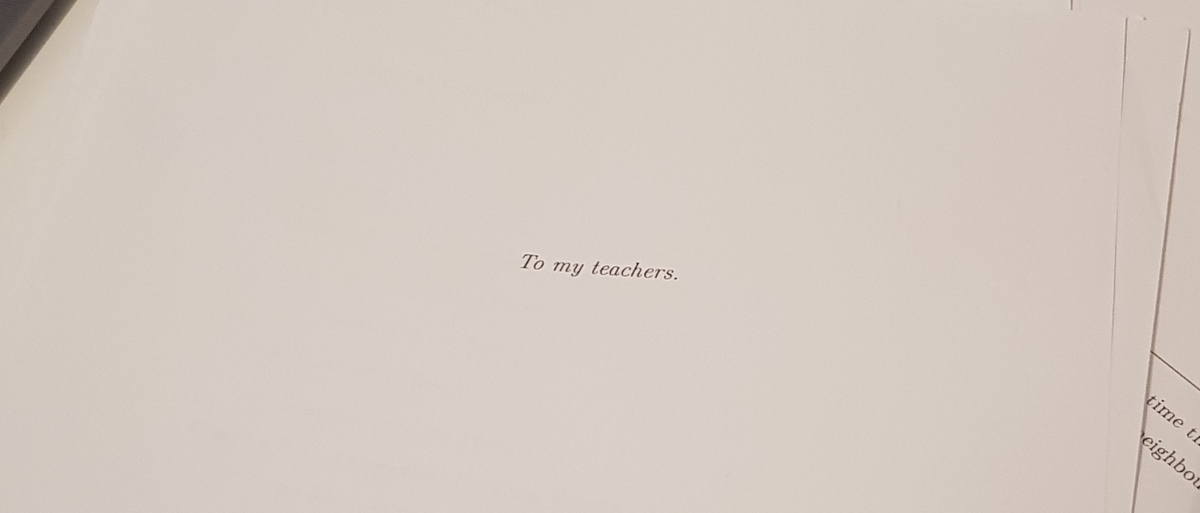
\includegraphics[width=\framewidth,height=\textheight,keepaspectratio]{tomyteachers.png}

	\note{%
		Nombrar a:

		Noemí, Pablo Coll, Charles, Agustín (coach), el equipo de la ICPC, Mamá, Papá, Reneé, Mauricio, los profesores y ayudantes de Exactas, Gravano, los jurados, Feuerstein, Grandata, Yannick.
	}
\end{frame}

\section{Preguntas}
\subsection{Preguntas}
\begin{frame}
	\centering
	\Huge ¿Preguntas?
\end{frame}

\end{document}
